%%%%%%%%%%%%%%%%%%%%%%%%%%%%%%%%%%%%%%%%%
% Masters/Doctoral Thesis 
% LaTeX Template
% Version 2.3 (25/3/16)
%
% This template has been downloaded from:
% http://www.LaTeXTemplates.com
%
% Version 2.x major modifications by:
% Vel (vel@latextemplates.com)
%
% This template is based on a template by:
% Steve Gunn (http://users.ecs.soton.ac.uk/srg/softwaretools/document/templates/)
% Sunil Patel (http://www.sunilpatel.co.uk/thesis-template/)
%
% Template license:
% CC BY-NC-SA 3.0 (http://creativecommons.org/licenses/by-nc-sa/3.0/)
%
%%%%%%%%%%%%%%%%%%%%%%%%%%%%%%%%%%%%%%%%%

%----------------------------------------------------------------------------------------
%	PACKAGES AND OTHER DOCUMENT CONFIGURATIONS
%----------------------------------------------------------------------------------------

\documentclass[
11pt, % The default document font size, options: 10pt, 11pt, 12pt
%oneside, % Two side (alternating margins) for binding by default, uncomment to switch to one side
%chapterinoneline,% Have the chapter title next to the number in one single line
%english, % ngerman for German
spanish,
singlespacing, % Single line spacing, alternatives: onehalfspacing or doublespacing
%draft, % Uncomment to enable draft mode (no pictures, no links, overfull hboxes indicated)
%nolistspacing, % If the document is onehalfspacing or doublespacing, uncomment this to set spacing in lists to single
%liststotoc, % Uncomment to add the list of figures/tables/etc to the table of contents
%toctotoc, % Uncomment to add the main table of contents to the table of contents
parskip, % Uncomment to add space between paragraphs
%nohyperref, % Uncomment to not load the hyperref package
headsepline, % Uncomment to get a line under the header
]{MastersDoctoralThesis} % The class file specifying the document structure



\usepackage{pstricks,pst-node} %diagramas de flujo
%para los diagramas de flujo y definir el stilo
\usepackage{tikz}
\usetikzlibrary{shapes.geometric, arrows}
\tikzstyle{startstop} = [rectangle, rounded corners, minimum width=3cm, minimum height=1cm,text centered, draw=black, fill=red!30]

\tikzstyle{io} = [trapezium, trapezium left angle=70, trapezium right angle=110, minimum width=3cm, minimum height=1cm, text centered, draw=black, fill=blue!30]

\tikzstyle{process} = [rectangle, minimum width=3cm, minimum height=1cm, text centered,text width=3cm, draw=black, fill=orange!30]
\tikzstyle{decision} = [diamond, minimum width=3cm, minimum height=1cm, text centered, text width=1.5cm, draw=black, fill=green!30]

\tikzstyle{fsm} = [circle,inner sep=0pt, text centered,draw=black, fill=blue!30]

\tikzstyle{arrow} = [thick,->,>=stealth]
\tikzset{
error/.style = {circle, draw, fill=red, align=center,
                inner sep=0pt},
                }
%.---------------------------------------------------
\usepackage{float} % para H en las figuras
\usepackage[utf8]{inputenc} % Required for inputting international characters
\usepackage[T1]{fontenc} % Output font encoding for international characters

\usepackage{palatino} % Use the Palatino font by default
%,style=authoryear
%\usepackage[backend=bibtex,natbib=true]{biblatex} % Use the bibtex backend with the authoryear citation style (which resembles APA)
\usepackage[backend=biber,style=numeric,sorting=none,natbib=true]{biblatex}
%\usepackage[backend=biber,style=numeric,sorting=none]{biblat‌​ex}
\addbibresource{references.bib} % The filename of the bibliography

\usepackage[autostyle=true]{csquotes} % Required to generate language-dependent quotes in the bibliography

\usepackage{caption}
\usepackage{subcaption}

%------------------------
\usepackage{listings}

%\usepackage[hyphens]{url}
%\usepackage[hidelinks]{hyperref}
%\hypersetup{breaklinks=true}
\urlstyle{same}
%\usepackage{cite}

%--------------------------

\usepackage{color}

%
%----------------------------------------------------------------------------------------
%	MARGIN SETTINGS
%----------------------------------------------------------------------------------------

\geometry{
	paper=a4paper, % Change to letterpaper for US letter
	inner=2cm, % Inner margin
	outer=3.3cm, % Outer margin
	bindingoffset=2cm, % Binding offset
	top=1.5cm, % Top margin
	bottom=1.5cm, % Bottom margin
	%showframe,% show how the type block is set on the page
}

%----------------------------------------------------------------------------------------
%	INFORMACIÓN DE LA MEMORIA
%----------------------------------------------------------------------------------------

\thesistitle{Dispositivo logger IoT con tecnologías de comunicación Sigfox y Lora} % El títulos de la memoria, se usa en la carátula y se puede usar el cualquier lugar del documento con el comando \ttitle
\supervisor{Ing. Marcelo E. Romeo (UNSAM, UTN-FRBA)} % El nombre del director, se usa en la carátula y se puede usar el cualquier lugar del documento con el comando \supname
\degree{Especialista en Sistemas Embebidos } % Nombre del grado, se usa en la carátula y se puede usar el cualquier lugar del documento con el comando \degreename
\author{Ing. Julian Bustamante Narvaez} % Tu nombre, se usa en la carátula y se puede usar el cualquier lugar del documento con el comando \authorname
\juradoUNO{Esp. Ing. Leonardo Carducci (FIUBA)} % Nombre y pertenencia del un jurado se usa en la carátula y se puede usar el cualquier lugar del documento con el comando \jur1name
\juradoDOS{Esp. Ing. Agustin Bassi (FIUBA)} % Nombre y pertenencia del un jurado se usa en la carátula y se puede usar el cualquier lugar del documento con el comando \jur2name
\juradoTRES{Esp. Ing. Ramiro Alonso (FIUBA)} % Nombre y pertenencia del un jurado se usa en la carátula y se puede usar el cualquier lugar del documento con el comando \jur3name
\fechaINICIO{agosto de 2018}
\fechaFINAL{agosto de 2019}

\subject{Memoria del Trabajo Final de la Carrera de Especialización en Sistemas Embebidos de la UBA} % Your subject area, this is not currently used anywhere in the template, print it elsewhere with \subjectname
\keywords{CESE, Sistemas Embebidos, CIAA} % Keywords for your thesis, this is not currently used anywhere in the template, print it elsewhere with \keywordnames
\university{Universidad de Buenos Aires} % Your university's name and URL, this is used in the title page and abstract, print it elsewhere with \univname
\faculty{{Facultad de Ingeniería}} % Your faculty's name and URL, this is used in the title page and abstract, print it elsewhere with \facname
\department{Departamento de Electrónica} % Your department's name and URL, this is used in the title page and abstract, print it elsewhere with \deptname
\group{{Laboratorio de Sistemas Embebidos}} % Your research group's name and URL, this is used in the title page, print it elsewhere with \groupname


\hypersetup{pdftitle=\ttitle} % Set the PDF's title to your title
\hypersetup{pdfauthor=\authorname} % Set the PDF's author to your name
\hypersetup{pdfkeywords=\keywordnames} % Set the PDF's keywords to your keywords


\newcaptionname{spanish}{\acknowledgementname}{Agradecimientos}
\newcaptionname{spanish}{\authorshipname}{Declaración de Autoría}
\newcaptionname{spanish}{\abbrevname}{Glosario}
\newcaptionname{spanish}{\byname}{por}

\renewcommand{\lstlistingname}{Algoritmo}% Listing -> Algorithm
\renewcommand{\lstlistlistingname}{Índice de \lstlistingname s}% List of Listings -> List of Algorithms

\renewcommand{\listtablename}{Índice de Tablas}
\renewcommand{\tablename}{Tabla} 

\addtolength{\footnotesep}{2mm} % Espacio adicional en los footnotes

\begin{document}

\frontmatter % Use roman page numbering style (i, ii, iii, iv...) for the pre-content pages

\pagestyle{plain} % Default to the plain heading style until the thesis style is called for the body content

%----------------------------------------------------------------------------------------
%	CARÁTULA
%----------------------------------------------------------------------------------------

\begin{titlepage}
\begin{center}

{\scshape\LARGE UNIVERSIDAD DE BUENOS AIRES\par}\vspace{0.1cm} % University name
{\scshape\LARGE FACULTAD DE INGENIERÍA\par}\vspace{0.1cm} % Faculty name
{\scshape\LARGE Carrera de Especialización en Sistemas Embebidos\par}\vspace{1cm} % Thesis type

\includegraphics[width=.3\textwidth]{./Figures/logoFIUBA.png}
\vspace{1cm}

\textsc{\Large Memoria del Trabajo Final}\\[0.5cm] % Thesis type

{\huge \bfseries \ttitle\par}\vspace{0.4cm} % Thesis title

\vspace{1cm}
\LARGE\textbf{Autor:\\
\authorname}\\ % Author name

\vspace{1cm}

\large
\vspace{10px}
{Director:} \\
{\supname} % Supervisor name
 
\vspace{1cm}
Jurados:\\
\jurunoname\\
\jurdosname\\
\jurtresname
 
\vfill
\textit{Este trabajo fue realizado en la Ciudad Autónoma de Buenos Aires, entre \fechaINICIOname \hspace{1px} y \fechaFINALname.}
\end{center}
\end{titlepage}


%----------------------------------------------------------------------------------------
%	RESUMEN - ABSTRACT 
%----------------------------------------------------------------------------------------

\begin{abstract}
\addchaptertocentry{\abstractname} % Add the abstract to the table of contents
%
%The Thesis Abstract is written here (and usually kept to just this page). The page is kept centered vertically so can expand into the blank space above the title too\ldots
\centering

En esta memoria se presenta el diseño e implementación de un dispositivo de adquisición de datos con múltiples entradas digitales y análogicas para aplicaciones IoT (\textit{Internet of Things}) en ambientes industriales
para la empresa Tecrea S.A.S. El dispositivo tiene una arquitectura modular que le permite incorporar nuevas funcionalidades y puede operar con protocolos
inalámbricos como SigFox o Lora.

Este proyecto se enfocó en que los procesos de toma de datos sean menos dependientes de las personas y se puedan auto gestionar con información
adquirida en tiempo real.
En el presente trabajo se plasman los conocimientos en el desarrollo de firmware en sistemas embebidos, 
testing de software, diseño electrónico, circuitos impresos y gestión de proyectos.

\end{abstract}

%----------------------------------------------------------------------------------------
%	CONTENIDO DE LA MEMORIA  - AGRADECIMIENTOS
%----------------------------------------------------------------------------------------

\begin{acknowledgements}
%\addchaptertocentry{\acknowledgementname} % Descomentando esta línea se puede agregar los agradecimientos al índice
\vspace{1.5cm}

A la mujer de mi vida, Adriana, por el sacrificio que hizo y la comprensión que tuvo en los momentos donde no tenía tiempo para ella.

A mi madre Edith, a mi padre Oscar y a mis hermanos, Lina, Jonatan, Felipe y Melissa por la ayuda imprescindible, por creer en mis expectativas y por comprender mis largas horas de trabajo y estudio. 

A Tecrea SAS por el tiempo y colaboración brindada y a cada uno de mis compañeros de trabajo por todas sus enseñanzas.

\end{acknowledgements}

%----------------------------------------------------------------------------------------
%	LISTA DE CONTENIDOS/FIGURAS/TABLAS
%----------------------------------------------------------------------------------------
\renewcommand{\listtablename}{Índice de Tablas}

\tableofcontents % Prints the main table of contents

\listoffigures % Prints the list of figures

\listoftables % Prints the list of tables


%----------------------------------------------------------------------------------------
%	CONTENIDO DE LA MEMORIA  - DEDICATORIA
%----------------------------------------------------------------------------------------

\dedicatory{\textbf{
Con paciencia, dedicación y perseverancia los sueños se pueden cumplir.
Este trabajo se lo dedico a toda familia, ellos son el motor de mis sueños. }}  % escribir acá si se desea una dedicatoria

%----------------------------------------------------------------------------------------
%	CONTENIDO DE LA MEMORIA  - CAPÍTULOS
%----------------------------------------------------------------------------------------

\mainmatter % Begin numeric (1,2,3...) page numbering

\pagestyle{thesis} % Return the page headers back to the "thesis" style

\renewcommand{\tablename}{Tabla} 

% Incluir los capítulos como archivos separados desde la carpeta Chapters
% Descomentar las líneas a medida que se escriben los capítulos

% Chapter 1

\chapter{Introducción General} % Main chapter title
En este capítulo se menciona la problemática que motivó la realización del presente trabajo, los procedimientos de la toma de datos en la industria actualmente y el enfoque elegido para desarrollar el prototipo que ofrece una solución usando sistemas embebidos.
\label{Chapter1} % For referencing the chapter elsewhere, use \ref{Chapter1} 
\label{IntroGeneral}

%----------------------------------------------------------------------------------------

% Define some commands to keep the formatting separated from the content 
\newcommand{\keyword}[1]{\textbf{#1}}
\newcommand{\tabhead}[1]{\textbf{#1}}
\newcommand{\code}[1]{\texttt{#1}}
\newcommand{\file}[1]{\texttt{\bfseries#1}}
\newcommand{\option}[1]{\texttt{\itshape#1}}
\newcommand{\grados}{$^{\circ}$}

%----------------------------------------------------------------------------------------

%\section{Introducción}

%----------------------------------------------------------------------------------------
\section{Motivación}
En el transcurso de la próxima década se espera un gran crecimiento en la cantidad de dispositivos IoT (\textit{internet of things}) provenientes de redes LPWAN (\textit{Low-Power Wide Area Network}). Para el 2025, se espera que más de 100 billones de dispositivos se conecten a través de LPWAN\cite{taylor2015world}. Las principales tecnologías, que prometen una vida útil alta de la batería de los dispositivos y un alcance de hasta 15 kilómetros, son Sigfox, Lora y NB-IoT, que actualmente están conectados en todo el mundo con más de 25 millones de dispositivos, brindando servicio y facilitando las experiencias del usuario\citep{iotanalytics}.

En los procesos industriales se tiene mucha información de variables físicas y eléctricas por medio de sensores, la cual muchas veces no se aprovecha debido a que no se tiene una óptima trazabilidad de la misma o simplemente se pierde esta información. Cuando los procesos industriales fallan, necesitan una reacción inmediata por parte de una persona y esto genera una dependencia de alguien que no siempre va a estar las 24 horas del día al pendiente, quizá por costos para las mismas empresas.

En vista de lo de anterior se desarrolló un prototipo para ofrecer una solución que permita monitorear inalambricamente diferentes variables en los procesos industriales de esta manera los usuarios pueden estar informados y garantizan la correcta funcionalidad de sus procesos.

%https://iot-analytics.com/state-of-the-iot-update-q1-q2-2018-number-of-iot-devices-now-7b/


\section{IoT (\textit{Internet of Things})}
El concepto de internet de las cosas se refiere a la interconexión digital de dispositivos y objetos  a través  de una red, es decir, dispositivos como sensores y/o actuadores, equipados con una interfaz de comunicación, unidades de procesamiento y almacenamiento\cite{centenaro2016long}. Estos dispositivos tienen la capacidad de adquirir, intercambiar y transferir datos a la red mediante alguna tecnología de comunicación inalámbrica.



IoT es una tendencia imparable y puede facilitar mucho la vida diaria. Produce formas baratas y efectivas de resolver grandes problemas sociales, como el acceso a la energía, el transporte y la vivienda. Otras aplicaciones pueden ser \textit{wearables}, construcciones y demóticas, \textit{smart cities}, \textit{smart manufacturing}\citep{taylor2015world}. IoT puede hacernos sentir más cómodos en nuestros hogares y en nuestras ciudades.

\subsection{Tecnologías de comunicación}
Uno de los principales habilitadores de un proyecto de internet de las cosas son las redes de comunicaciones. Estas permiten conectar dispositivos, máquinas, sensores o “cosas” los cuales generan datos o información desde cualquier punto geográfico del planeta. Las redes de comunicación son un conjunto de medios técnicos que permiten la comunicación entre equipos que se encuentran a distancia.

Las principales características de una red de comunicación IoT son:
\begin{itemize}
	\item Baja tasa de datos.
	\item Bajo consumo de energía.
	\item Largo alcance de comunicación.
	\item Conexiones bidireccionales.
	\item Movilidad y servicios de localización.

\end{itemize}

En la tabla \ref{tab:Tecno} se puede observar una comparación de las principales tecnologías de comunicación.

\begin{table}[h]
	\centering
	\caption[Redes de comunicación]{Redes de comunicación más utilizadas para proyectos IoT}
	\begin{tabular}{l c c c}    
		\toprule
		\textbf{Tecnología} 	 & \textbf{Consumo}  & \textbf{Alcance} 	& \textbf{Tasa de Datos} \\
		\midrule
		GSM/GPRS				 & Muy alto			& Alto					&	Alta \\		
		SigFox					 & Bajo				& Medio/alto			&	Muy baja \\
		Lora					 & Bajo				& Medio/alto			&	Muy baja\\	
		WiFi					 & Alto				& Bajo					&	Muy alta \\
		BLE					 	 & Muy bajo			& Muy Bajo				&	Baja \\
		ZigBee					 & Medio			& Bajo					&	Baja \\	
		\bottomrule
		\hline
	\end{tabular}
	\label{tab:Tecno}
\end{table}

\textbf{Tecnología GSM/GPRS:}

GSM (\textit{Global System for Mobile communications)} o en español sistema global para las comunicaciones móviles y es un tipo de red que se utiliza para la transmisión móvil de voz y datos.

GPRS (\textit{General Packet Radio Service)} o en español servicio general de paquetes vía radio y es una extensión mejorada del GSM.
Permite la mensajería instantánea, los servicios de mensajes cortos SMS (\textit{Short Message Service}), multimedia MMS (\textit{Multimedia Messaging Service}) y correo electrónico. Esta proporciona una cobertura inalámbrica completa, tiempos de acceso mas cortos y mayores tasas de datos\citep{bettstetter1999gsm}. Por ejemplo, permite enviar 30 SMS por minuto, mientras que con GSM se puede enviar entre 6 y 10.

\textbf{Tecnología WiFi:}

Es una tecnología que permite la interconexión inalámbrica de dispositivos electrónicos por medio de internet. WiFi, el nombre popular para el área local inalámbrica Redes basadas en el estándar IEEE 802.11b, se ha convertido en la Tecnología preferida para redes inalámbricas de área local en entornos comerciales y domésticos\citep{henry2002wifi}.

\textbf{Tecnología BLE:}

Es una tecnología de red de área personal PAN (\textit{Personal Area Network}) inalámbrica, Permite la comunicación entre dispositivos dos o  más dispositivos Bluetooth, que opera en 2.4 GHz (una de las bandas ISM), con una tasa de transferencia de 1 Mbps en la capa física. BLE (\textit{Bluetooth Low Energy}) se introdujo por primera vez en 2010 con el objetivo de expandir la aplicación de Bluetooth para su uso en dispositivos con limitaciones de energía, como los inalámbricos. Sensores y controles inalámbricos. Los sensores y controles requieren un bajo consumo de energía, pero la cantidad de transmisión de datos es pequeña y la comunicación ocurre con poca frecuencia\citep{chang2014bluetooth}.


\textbf{Tecnología ZigBee:}

ZigBee es uno de El transceptor estándar más utilizado en sensores inalámbricos.redes ZigBee sobre IEEE 802.15.4 , define especificaciones para baja velocidad de datos WPAN (\textit{wireless personal area network}) para soportar baja potencia en monitorización y control de dispositivos\citep{ramya2011study}.

El consumo de energía para ZigBee es muy pequeño. En la mayoría de los casos Utiliza 1mW (o menos potencia). Pero aún así proporciona un alcance hasta 150 metros en exterior que se consigue con la técnica.llamado espectro de propagación de secuencia directa DSSS (\textit{direct sequence spread spectrum}).Funciona en los 868 MHz (Europa), 915 MHz (América del Norte y Australia) y 2.4 GHz (disponible en todo el mundo) banda ISM con hasta 20kbps, 40kbps y velocidad de datos de 250kbps respectivamente\citep{ramya2011study}.

\textbf{Tecnología NB-IoT (\textit{Narrowband Internet of Things}:}

Tecnología de acceso por radio que proporciona cobertura extendida, alta capacidad y larga duración de la batería. Utiliza la ya existente red móvil para conectar dispositivos de manera masiva.

NB-IoT requiere un ancho de banda mínimo de 180 kHz, que es igual al tamaño del LTE físico más pequeño.
Dependiendo de la disponibilidad del espectro, esta tecnología se puede implementar por sí solo en los portadores de guardia de LTE / UMTS existentes\citep{adhikary2016performance}.

\textbf{Tecnología LTE-M:}

Es un tipo de tecnología de radio de red LPWAN que permite una amplia gama de dispositivos celulares y servicios (específicamente, para aplicaciones de máquina a máquina e IoT). Utiliza la ya existente red móvil para conectar dispositivos de manera masiva.

\textbf{Tecnología SigFox:} 

Es una tecnología de comunicación UNB (\textit{Ultra-Narrow Band}) para conectar sensores y dispositivos. Opera en las bandas 868 MHz y 902-928 MHz.

\textbf{Tecnología LoRa:} 

Es una tecnología LPWAN de modulación de radio de CCS (\textit{chirp spread spectrum}). Esta permite el envió y recepción de información en las bandas de frecuencia 433 MHz, 868 MHZ y 915 MHz .

%---------------Objetivos y alcance 
\section{Objetivos y alcance}

\subsection{Objetivo}
El objetivo principal es diseñar e implementar un dispositivo de adquisición de datos con múltiples entradas digitales y analógicas para aplicaciones IoT en ambientes industriales, mediante la transmisión inalámbrica de la información por medio de tecnologías de comunicación Sigfox o Lora. 

\subsection{Alcance}

En la presente solución se contempla:


\begin{itemize}
	\item La implementación de un prototipo funcional de hardware.
	\item 2 entradas analógicas de tensión.
	\item 1 entrada analógica de corriente.
	\item 5 entradas digitales.
	\item La escritura del firmware del dispositivo.
	\item La transmisión de la información por medio de Sigfox.
	\item La transmisión de la información por medio de Lora.
	\item La visualización de la información en una plataforma paga o libre.
	\item Se incluye partes del código de la biblioteca usada para el modulo Sigfox.
\end{itemize}
En la presente solución no se contempla:
\begin{itemize}
	\item El desarrollo de la plataforma web que permite visualizar los datos en linea.
	\item Caja plástica del dispositivo.
\end{itemize}
En la presente solución no se incluye:
\begin{itemize}
	\item Diagramas esquemáticos.
	\item PCB \textit{layout}.
	\item Firmware.
\end{itemize}

Esto debido a que la propiedad intelectual es de Tecrea SAS.


%----------------------------------------------------------------------------------------


\chapter{Introducción Específica} % Main chapter title

\label{Chapter2}

%----------------------------------------------------------------------------------------
%	SECTION 1
%----------------------------------------------------------------------------------------
En este capitulo se presenta la idea general del proyecto y se describen las características principales de la solución implementada.
\section{Estructura general del sistema}

%\label{sec:ejemplo}

El diagrama general del sistema se muestra en figura \ref{fig:esquemaGeneral}. El sistema se compone de un microcontrolador ARM(\textit{Advanced RISC Machine}) Cortex\textregistered -M4 y dos bus UART(\textit{Universal Asynchronous Receiver-Transmitter}). De esta forma el sistema puede tener una arquitectura modular que le permite incorporar nuevas tecnologías de comunicación para transmitir inalambricamente tales como: SigFox, LoRa, Nb-IOT, Cat-M, WiFi y 3G.


\begin{figure}[h]

	\centering

	\includegraphics[scale=.35]{./Figures/esquemaGeneral.png}

	\caption{Diagrama general del sistema.}

	\label{fig:esquemaGeneral}

\end{figure}


El sistema consta dos entradas analógicas de tensión, una de corriente y cinco entradas digitales con el fin de poder adquirir datos de diferentes variables en los procesos industriales. El dispositivo esta diseñado para tener diferentes funcionalidades sin embargo debido a la delimitación del alcance del trabajo no se implementaron los subsistemas que se observan en gris en la figura \ref{fig:esquemaGeneral}.

%https://www.sigfox.com/en/sigfox-iot-radio-technology
\section{Sigfox}
La tecnología Sigfox fue fundada en Francia en 2010 con el fin de construir una red global que se dedicara al Internet de las cosas y operara con un costo muy bajo y un consumo mínimo de energía. La tecnología Sigfox se basa en una comunicación por radio de largo alcance, dedicada por completo a hacer que cualquier objeto se comunique con muy bajo consumo de energía, extrayendo y transportando mensajes muy pequeños \cite{SigfoxGlobalNetwork}.
%https://www.sigfox.com/en/sigfox-global-iot-network

%https://build.sigfox.com/sigfox#coverage
El protocolo Sigfox se centra en: 
\begin{itemize}
    \item Autonomía: consumo de energía extremadamente bajo, lo que permite años de duración de la batería.
    \item Simplicidad:  sin configuración, solicitud de conexión o señalización. ¡El dispositivo está en funcionamiento en minutos!
    \item Eficiencia de precio: desde el hardware utilizado en los dispositivos hasta la red, optimiza cada paso para que sea lo más rentable posible.
    \item Pequeños mensajes: no permiten activos o medios grandes en la red, solo notificaciones pequeñas: hasta 12 bytes en transmisiones ascendentes y 8 bytes transmisiones descendentes.
    \item Complementariedad: gracias al bajo costo y facilidad de configuración, también se puede usar Sigfox como una solución secundaria para cualquier otro tipo de red, como: WiFi, Bluetooth, GPRS, etc.
\end{itemize}

Como se puede observar en la figura \ref{fig:SigfoxOverview} el ciclo de vida de un mensaje de Sigfox es el siguiente:
\begin{enumerate}
    \item Un dispositivo se despierta y emite un mensaje usando su antena de radio.
    \item Múltiples estaciones base de Sigfox en el área reciben el mensaje.
    \item Las estaciones base envían el mensaje a la nube de Sigfox.
    \item La nube de Sigfox envía el mensaje a la plataforma de el cliente.
\end{enumerate}

\begin{figure}[h]
	\centering
	\includegraphics[scale=.25]{./Figures/SigfoxOverview.jpg}
	\caption{Ciclo de vida de un mensaje en Sigfox\protect\footnotemark.}
	\label{fig:SigfoxOverview}
\end{figure}


Sigfox utiliza la tecnología de radio UNB y opera en las bandas sin licencia ISM (\textit{industrial, scientific and medical}) para intercambiar mensajes de radio a través del aire en las frecuencias 868 MHz y 902-928 MHz. En cada pais, las  bandas ISM están bajo el control de las regulaciones locales, que definen restricciones técnicas para el uso del espectro, Sigfox tiene definidas configuraciones de radio que cumplan con las regulaciones locales.

%La modulación por desplazamiento de fase o PSK (Phase Shift Keying) es una forma de modulación angular que consiste en hacer variar la fase de la portadora entre un número determinado de valores discretos. La diferencia con la modulación de fase convencional (PM) es que mientras en ésta la variación de fase es continua, en función de la señal moduladora, en la PSK la señal moduladora es una señal digital y, por tanto, con un número de estados limitado.%

%https://www.link-labs.com/blog/sigfox-vs-lora
Sigfox combina UNB con modulación  DBPSK (\textit{differential binary phase shift keying}), este un método de transmisión de radio estándar que toma fragmentos de espectro muy estrechos y cambia la fase de la onda de radio portadora para codificar los datos. Esto permite que el receptor solo escuche en una pequeña porción de espectro. Lo que mitiga el efecto del ruido. cada mensaje tiene un ancho de 100 Hz y se transfiere a una velocidad de 100 o 600 bits por segundos, dependiendo de la región \citep{RSpec}.

%https://build.sigfox.com/sigfox-device-radio-specifications

Tiene una funcionalidad bidireccional, pero la capacidad para ir desde la estación base hasta el dispositivo final está restringida, y tendrá menos presupuesto de enlaces que hacia abajo. Esto se debe a que la sensibilidad del receptor en el dispositivo final no es tan buena como en la estación base.

%https://build.sigfox.com/sigfox-radio-configurations-rc
Sigfox tiene una red de cobertura global, que opera en la banda ISM en todo el mundo. Las operaciones globales se dividen actualmente en seis zonas geográficas. Cada zona tiene un conjunto diferente de parámetros que acotan claramente la implementación del hardware del dispositivo, principalmente rango de frecuencias, frecuencia central(Fc) y potencia máxima irradiada. En la tabla \ref{tab:ZonasSigfox} se puede observar algunos de estos parámetros \citep{RConfg}.
\footnotetext{\url{https://build.sigfox.com/sigfox}}
\begin{table}[h]
    \small
	\centering
	\caption[Zonas de frecuencia]{Frecuencias según zonas}
	\begin{tabular}{l c c c c c c}    
		\toprule
		\textbf{ } 	   & \textbf{RC1} & \textbf{RC2} 	& \textbf{RC3}  & \textbf{RC4}   & \textbf{RC5}	& \textbf{RC6} \\
		\midrule
		Fc \textit{uplink} (MHz)	    & 868.130 	& 902.200	&923.200  &920.800	&923.300 &865.200\\	
		Fc \textit{downlink} (MHz) 	& 869.525	& 905.200   &922.200 &922.300	&922.300	&866.300\\
		Velocidad \textit{uplink} (bits/s)	& 100       &600        &100     &600       &100        &100\\	
		Velocidad \textit{downlink} (bits/s)	& 600       & 600    	&600     & 600       & 600    	&600\\
		EIRP (dBm)		                             	 & 16       & 24		&16     &24	        &14         &16\\
		\bottomrule
		\hline
	\end{tabular}
	\label{tab:ZonasSigfox}
\end{table}

Las 6 zonas  actuales con la configuración de radio de Sigfox son:
\begin{itemize}
    \item RC1:
        \begin{itemize}
            \item Europa: Bélgica, Croacia, República Checa, Dinamarca, Estonia, Finlandia, Francia, Alemania, Hungría, Irlanda, Italia, Luxemburgo, Malta, Países Bajos, Noruega, Polonia, Portugal, Eslovaquia, España, Suecia, Suiza, Reino Unido.
            \item Francia de ultramar: Guayana Francesa, Polinesia Francesa, Guadalupe, Martinica, Mauricio, Mayotte, Nueva Caledonia, Reunión.
            \item Oriente Medio y África: Irán, Kenia, Omán, Sudáfrica, Túnez, Emiratos Árabes Unidos.
        \end{itemize}
    \item RC2: Brasil, Canadá, México, Puerto Rico, Estados Unidos.
    \item RC3: Japón
    \item RC4:
        \begin{itemize}
            \item América Latina: Argentina, Chile, Colombia, Costa Rica, Ecuador, El Salvador, Guatemala, Honduras, Panamá, Perú, Uruguay.
            \item Asia Pacífico: Australia, Hong Kong, Malasia, Nueva Zelanda, Singapur, Taiwán, Tailandia.
        \end{itemize}
    \item RC5: Corea del Sur
    \item RC6: India

\end{itemize}

En la figura \ref{fig:coverageSigfox} se puede observar el mapa de cobertura de Sigfox.

\begin{figure}[h]
	\centering
	\includegraphics[scale=.65]{./Figures/coverageSigfox.PNG}
	\caption{Disponibilidad geográfica de Sigfox\protect\footnotemark.}
	\label{fig:coverageSigfox}
\end{figure}
\footnotetext{\url{https://build.sigfox.com/sigfox-radio-configurations-rc}}
%https://build.sigfox.com/certification
La certificación Sigfox es el reconocimiento de la conformidad de un dispositivo con las especificaciones de certificación Sigfox para garantizar la compatibilidad con los servicios Sigfox y el rendimiento nominal en la red. La certificación Sigfox \textit{Ready} es obligatoria para que cualquier dispositivo esté conectado a la red Sigfox, con la excepción de las soluciones de desarrollo (prototipos).

Sigfox requiere la certificación para los dispositivos que desean comunicarse en la red Sigfox. Esto es para garantizar la interoperabilidad y la prestación de servicios a un nivel de rendimiento nominal. Al finalizar el proceso de certificación, Sigfox otorga un certificado al cliente. Este certificado es necesario para registrar cualquier dispositivo del mismo modelo en la red Sigfox.

La certificación Sigfox \textit{Ready} se clasifica en clases. RC (\textit{Radio Configuration}) es la zona de configuración, la cual depende de la región. En la tabla \ref{tab:ZonasSigfox} se observan las características\citep{CertificationSigfox}.
%https://storage.sbg1.cloud.ovh.net/v1/AUTH_669d7dfced0b44518cb186841d7cbd75/dev_medias/build/40599x1josfx0hz/Sigfox%20device%20cookbook%20-%20communication%20configuration%20Nov%202018.pdf
\begin{table}[h]
	\centering
	\caption[Sigfox \textit{Ready}]{Caracteristicas de certificación (\textit{Sigfox Device Class}) }
	\begin{tabular}{l c c c}    
		\toprule
		\textbf{  } & \multicolumn{3}{c}{\textit{Device EIRP}} \\ \cline{2-4} 
		\textbf{ \textit{Device Class} } & \textbf{RC1, RC3} & \textbf{RC2,RC4} 	& \textbf{RC5} \\
		\midrule
		0u	    &$\ge12$ dBm 	&$\ge20$ dBm & $\ge10$ dBm \\	
		1u	&$\ge7$ and <12 dBm &$\ge15$ and <20 dBm & $\ge5$ and <10 dBm\\
		2u	&$\ge2$ and <7 dBm & $\ge10$ and <15 dBm & $\ge0$ and <5 dBm \\	
		3u	&< 2 dBm &< 10 dBm &< 0 dBm   \\
		\bottomrule
		\hline
	\end{tabular}
	\label{tab:ZonasSigfox}
\end{table}
%https://storage.sbg1.cloud.ovh.net/v1/AUTH_669d7dfced0b44518cb186841d7cbd75/dev_medias/build/40599x1josfx0hz/Sigfox%20device%20cookbook%20-%20communication%20configuration%20Nov%202018.pdf

La figura \ref{fig:certificacion} muestra la prioridad de las clases, siendo clase 0u la de mayor potencia de transmisión y 3u la clase de menor potencia de transmisión. Entre mayor potencia mayor alcance se puede tener con el dispositivo\citep{CertificationSigfox}.
\begin{figure}[h]
	\centering
	\includegraphics[scale=.65]{./Figures/certificacion.PNG}
	\caption{Potencia según clases.}
	\label{fig:certificacion}
\end{figure}

%https://www.sigfox.com/en/coverage 
Sigfox se basa en una infraestructura privada de antenas y servidores, la red es desplegada por un operador local. En América es la empresa WND \textit{group } (\textit{Wireless Network Development}) con exclusividad por 15 años. Sin embargo en otros partes del mundo son otras empresas las encargadas de desplegar la red. WND se encuentra en Colombia, Argentina, Brasil, Chile, Costa Rica, Ecuador, El Salvador, Mexico, Panamá y United Kingdom. También existen los canales que son los encargados de consumir y ofrecer el servicio que brinda WND \citep{SigfoxCoverage}. 
%https://build.sigfox.com/backend-callbacks-and-api

La información se maneja en un servidor Sigfox  \textit{back-end} donde el usuario tiene la posibilidad darle un tratamiento a la información a través de una interfaz API (\textit{Application Programming Interface}). En la plataforma de Sigfox, una empresa suele estar representada por un "Grupo", que contiene "Tipo de dispositivo". Cada tipo de dispositivo puede atribuirse a una "familia" de dispositivos como se observa en la figura \ref{fig:backendSigfox}. Todas las unidades del mismo producto se agruparán como un tipo de dispositivo para permitir que todas se comporten exactamente de la misma manera cuando la red Sigfox recibe un mensaje. 
%https://build.sigfox.com/backend-callbacks-and-api
\begin{figure}[h]
	\centering
	\includegraphics[scale=.35]{./Figures/backendSigfox.jpg}
	\caption{Diagrama Sigfox \textit{back-end} \protect\footnotemark}
	\label{fig:backendSigfox}
\end{figure}
\footnotetext{\url{https://build.sigfox.com/backend-callbacks-and-api}}

Sigfox basa su modelo de negocio en conectividad, ofrece servicios de comunicación seguros, bidireccionales y listos para usar, para conectar los dispositivos a la nube. Existen planes de conectividad anuales que difieren en la cantidad de mensajes que pueden transmitir al día (ver figura \ref{fig:PlanesSigfox}). Por ejemplo un plan \textit{platinium}, tiene máximo 140 mensajes \textit{uplink} y 4 mensajes \textit{downlink}. Los mensajes de bajada (\textit{downlink}) siempre están precedidos por un mensaje ascendente. En cualquier otro momento que el servidor quiera enviar un mensaje descendente debe esperar hasta la siguiente transmisión de un mensaje ascendente (\textit{uplink}).

El costo para el plan \textit{platinium} se puede observar en la figura \ref{fig:CostoSigfox}. Se puede apreciar que son 2.625 USD por crear el dispositivo, 2.625 USD por activar el dispositivo y 5.25 USD por subscripción anual, donde los primeros tres años solo se pagaría este ultimo valor de subscripción por cada dispositivo por conectividad durante un año.

\begin{figure}[h]
	\centering
	\includegraphics[scale=.5]{./Figures/CostoSigfox.PNG}
	\caption{Costo plan \textit{platinium} para 100 dispositivos\protect\footnotemark}
	\label{fig:CostoSigfox}
\end{figure}
\footnotetext{\url{https://connect.sigfox.com/portal-web/views/quotes/simulation/simulation.xhtml}}
\begin{figure}[h]
	\centering
	\includegraphics[scale=.6]{./Figures/PlanesSigfox.PNG}
	\caption{Niveles de subscripción\protect\footnotemark}
	\label{fig:PlanesSigfox}
\end{figure}

%LoRa Alliance. White Paper: A Technical Overview of Lora and Lorawan; The LoRa Alliance: San Ramon, CA,USA, 2015.
\section{LoRa}
LoRa, el cual es el acrónimo de \textit{"Long Range"}, es un sistema de comunicaciones inalámbricas de largo alcance, originalmente fue desarrollada por Semtech y actualmente es promovida por LoRa \textit{Alliance}.

LoRa esta basada en dos capas distintas, como se puede observar en la figura \ref{fig:LoraStack}: 
\begin{enumerate}
    \item Capa física que utiliza la técnica de modulación  de radio CSS (\textit{Chirp Spread Spectrum})\citep{CSS}.
    \item LoRaWAN un protocolo de capa MAC (\textit{Medium Acces Control})\cite{LoRaAlliance2015}.
\end{enumerate}

\begin{figure}[h]
	\centering
	\includegraphics[scale=.55]{./Figures/LoraWanClasses.PNG}
	\caption{LoraWan Stack \textsuperscript{\ref{note1}}\citep{LoRaAlliance2015}.}
	\label{fig:LoraStack}
\end{figure}

\footnotetext{\url{https://connect.sigfox.com/portal-web/views/quotes/simulation/simulation.xhtml}}
% Text with first footnote\footnote{\label{note1}\url{https://lora-alliance.org/sites/default/files/2018-04/what-is-lorawan.pdf}}
% footnote\textsuperscript{\ref{note1}}.

%En las comunicaciones digitales, el espectro de propagación de chirrido ( CSS ) es una técnica de espectro ensanchado que utiliza pulsos de chirrido modulados en %frecuencia de banda ancha para codificar información. [1] Un chirrido es una señal sinusoidal de aumento o disminución de la frecuencia con el tiempo (a menudo con %una expresión polinomial para la relación entre el tiempo y la frecuencia). En la imagen se muestra un ejemplo de un cambio de tendencia en el que la frecuencia %aumenta linealmente con el tiempo. A veces, la frecuencia de los upchirps aumenta exponencialmente con el tiempo.
%Al igual que con otros métodos de espectro ensanchado, el espectro de chirrido utiliza todo su ancho de banda asignado para transmitir una señal, lo que lo hace %robusto al ruido del canal. Además, debido a que los chirridos utilizan una amplia banda del espectro, el espectro extendido de los chirridos también es resistente %al desvanecimiento de múltiples vías, incluso cuando se opera a una potencia muy baja. Sin embargo, es diferente del espectro extendido de secuencia directa (DSSS) %o del espectro expandido de salto de frecuencia (FHSS), ya que no agrega ningún elemento pseudoaleatorio a la señal para ayudar a distinguirlo del ruido en el %canal, sino que se basa en el Naturaleza lineal del pulso chirrido. Además, el espectro del chirrido es resistente al efecto Doppler., lo que es típico en %aplicaciones de radio móvil. [2]

La capa física LoRa, permite aplicaciones de largo alcance, baja potencia y comunicaciones de bajo rendimiento. Opera en las bandas ISM de 433 MHz, 868 MHz o 915 MHz, esto depende de la región en la que se despliegue la red. La carga útil de cada transmisión puede oscilar entre 2 y 255 octetos. La velocidad de datos puede alcanzar hasta 50 Kbps. Cuando se emplea la adición de canales. Esta técnica de modulación es una tecnología patentada por Semtech\citep{FEHRI20181096}.

%https://lora-alliance.org/sites/default/files/2018-05/2015_-_lorawan_specification_1r0_611_1.pdf
%LoraWanClasses.PNG

%LoRa Alliance. White Paper: A Technical Overview of Lora and Lorawan; The LoRa Alliance: San Ramon, CA,USA, 2015.
%https://www.tuv.com/media/corporate/products_1/electronic_components_and_lasers/TUeV_Rheinland_Overview_LoRa_and_LoRaWANtmp.pdf
LoRaWAN define el protocolo de comunicación y la arquitectura del sistema para la red mientras que la capa física LoRa permite el enlace de comunicación de largo alcance.
El protocolo y la arquitectura de red tienen la mayor influencia para determinar la duración de la batería de un nodo, la capacidad de la red, la calidad del servicio, la seguridad, y la variedad de aplicaciones servidas por la red\protect\footnote{\label{note1}\url{https://lora-alliance.org/sites/default/files/2018-04/what-is-lorawan.pdf}}. 


La arquitectura red es una topología estrella de largo alcance (\textit{star-of-stars}) en la que las puertas de enlace (\textit{gateways}) retransmiten los mensajes de los dispositivos finales. Es decir los nodos no están asociados con una puerta de enlace específica. En lugar, los datos transmitidos por un nodo normalmente son recibidos por múltiples puertas de enlace. Cada puerta de enlace reenviará el paquete recibido desde el nodo final al servidor de red a través de una interfaz de red de retorno (\textit{backhaul}) (ya sea 3G, Ethernet, satélite o WiFi). Ver figura \ref{fig:Loraarquitecturenetwork}.

\begin{figure}[h]
	\centering
	\includegraphics[scale=.65]{./Figures/Loraarquitecturenetwork.PNG}
	\caption{LoRa arquitectura de red\textsuperscript{\ref{note1}} \citep{LoRaAlliance2015}.}
	\label{fig:Loraarquitecturenetwork}
\end{figure}



La comunicación entre los nodos generalmente es bidireccional, la puerta de enlace se distrbuye en diferentes frecuencias, canales y tarifas de datos. Las tasas de datos de LoRa varían de 0.3 Kbps a 50Kbps, Para  maximizar la duración de batería de los dispositivos finales como la capacidad general de la red, la red LoRa gestiona la velocidad de datos y la salida de RF para cada dispositivo final individualmente\citep{Specification2015}.



Los dispositivos finales pueden transmitir en cualquier canal disponible en cualquier momento, siempre y cuando se respeten las siguientes reglas:
\begin{itemize}
    \item El dispositivo final cambia el canal de forma pseudoaleatoria para cada  transmisión. La diversidad de frecuencia resultante hace que el sistema sea más robusto para interferencias.
    \item El dispositivo final respeta el ciclo de trabajo de transmisión máximo en relación con los reglamentos de la sub-banda usados y locales.
    \item El dispositivo final respeta la duración máxima de transmisión (o tiempo de permanencia) en relación con la sub-banda utilizada y las normativas locales.
\end{itemize}

%FALATA HABLAR DE TEOREMA SHANON HARTLEY, ANCHO DE BANDA Y EL RUUIDO, SALTO DE FRECUENCIA Y DSSS EXPECTRO EXPANDIDO-SECUENCIA DIRECTA


\subsection{LoRaWAN Clases}

La red  LoRa distingue entre  tres clases bidireccionales: clase A, clase B, clase C. Estas tres clases se usan para diferentes aplicaciones y tienen una variedad de requisitos para optimizar una variedad de aplicaciones finales. Las clases intercambian la latencia de comunicación del enlace descendente frente a la duración de la batería. ver figura \ref{fig:Loracomparacionclases}.

\begin{figure}[h]
	\centering
	\includegraphics[scale=.45]{./Figures/Loracomparacionclases.PNG}
	\caption{LoraWan clases\protect\footnotemark. } %\textsuperscript{\ref{note1} \citep{LoRaAlliance2015}.}
	\label{fig:Loracomparacionclases}
\end{figure}
\footnotetext{\url{https://lora-alliance.org/sites/default/files/2018-04/what-is-lorawan.pdf}}

\begin{itemize}
    \item Clase A, bidireccional: los dispositivos finales de Clase A pueden programar una transmisión de enlace ascendente en función de las necesidades propias con una pequeña variación basada en una base de tiempo aleatorio (ALOHA -type of protocol), esta clase de dispositivos permite comunicaciones bidireccionales, por lo que a cada transmisión de enlace ascendente le siguen dos ventanas cortas de recepción. La transmisión del enlace descendente desde el servidor en cualquier otro momento tiene que esperar hasta que ocurra la siguiente transmisión de enlace ascendente. Los dispositivos de clase A tienen el menor consumo de energía, pero también ofrecen menos flexibilidad en las transmisiones de enlace descendente. Ver figura \ref{fig:LoraclassA}.

    \item Clase B, bidireccional con ranuras de recepción programadas: los dispositivos finales de Clase B  tienen ventanas extras de recepción  abiertos a unas horas programadas. Por lo tanto, se requiere una baliza sincronizada desde el servidor, de modo que
    El servidor pueda saber cuándo está escuchando el dispositivo final. Ver figura \ref{fig:LoraClaseB}.
    
    \item Clase C, bidireccional con ranuras de recepción máximas: los dispositivos finales de Clase C tienen casi todo el tiempo ventanas de recepción continuas, de esta forma tienen el máximo consumo de energía\protect\footnote{\label{note2}\url{https://upcommons.upc.edu/handle/2117/98853}}. Ver figura \ref{fig:LoraClaseC}. %RL: .
\end{itemize}


\begin{figure}[H]
	\centering
	\includegraphics[scale=.65]{./Figures/LoraclassA.PNG}
	\caption{Diagrama de un dispositivo clase A de LoRa\textsuperscript{\ref{note2}} \citep{Ruano2016}.}
	\label{fig:LoraclassA}
\end{figure}

\begin{figure}[H]
	\centering
	\includegraphics[scale=.75]{./Figures/LoraClaseB.PNG}
	\caption{Diagrama de un dispositivo clase B de LoRa\textsuperscript{\ref{note2}} \citep{Ruano2016}.}
	\label{fig:LoraClaseB}
\end{figure}


\begin{figure}[H]
	\centering
	\includegraphics[scale=.65]{./Figures/LoraClaseC.PNG}
	\caption{Diagrama de un dispositivo clase C de LoRa\protect\footnotemark \citep{Ruano2016}.} %\textsuperscript{\ref{note2}} 
	\label{fig:LoraClaseC}
\end{figure}
\footnotetext{\url{https://upcommons.upc.edu/handle/2117/98853}}


\section{Requerimientos}
Los siguientes son los requerimientos del presente trabajo:

\textbf{Grupo de requerimientos asociados al hardware:}
\begin{enumerate}

	\item Microcontrolador.

	\begin{itemize}

		\item Debe tener procesador ARM Cortex M4.

		\item Debe tener 3 puertos UART.

		\item Debe tener comunicación I2C/SPI.

		\item Debe tener memoria flash mayor a 64 kb.

		\item Debe tener 3 entradas analógicas.

		\item Debe tener 5 entradas digitales.

	\end{itemize}

	%\item Nivel de protección debe ser IP65.

	\item Módulo Sigfox.

		\begin{itemize}

			\item Debe tener un módulo \textit{Dual Zone} con comunicación por UART.

			\item Debe tener antena externa con centro de banda en 915 MHz.

		\end{itemize}

	\item Módulo Lora.

		\begin{itemize}

			\item Debe tener un módulo con comunicación por UART/I2C.

			\item Debe tener antena externa con centro de banda en 915 MHz.

		\end{itemize}

		\item El sistema debe tener una (1) entrada analógica de voltaje de 0-5 Vdc.
		
		\item El sistema debe tener una (1) entrada analógica de voltaje de 0-10 Vdc.

		\item El sistema debe tener una (1) entradas analógicas de corriente 4-20 mA.

		\item El sistema debe tener cuatro (4) entradas digitales 3.3-24 Vdc.

\end{enumerate}



\textbf{Grupo de requerimientos asociados al módulo Sigfox:}

	\begin{enumerate}

		\item Debe colocarse en modo de bajo consumo mientras no esté en uso.
		
		\item El consumo de corriente ser menor a 2.5 uA.

		\item Verificación de cada respuesta de comando AT enviado desde el MCU al módulo SigFox.

	\end{enumerate}





\textbf{Grupo de requerimientos asociados al módulo Lora:}

	\begin{enumerate}

		\item Verificación de cada respuesta de los comandos enviados desde el MCU al módulo Lora.

		\item Debe colocarse en modo de bajo consumo mientras no esté en uso.
		
		\item El consumo de corriente ser menor a 13 uA.

	\end{enumerate}



\textbf{Otros requerimientos:}

\begin{enumerate}

	\item En el sistema se podrán configurar umbrales máximos y mínimos de las lecturas analógicas.

	\item El sistema deberá verificar las entradas analógicas cada 1 minuto (parámetro configurable).

	\item El sistema saldrá del modo de bajo consumo cada vez que ocurra una interrupción por tiempo.

\end{enumerate}


%-----------------------------

% \subsection{Ecuaciones}
% \label{sec:Ecuaciones}

% Al insertar ecuaciones en la memoria estas se deben numerar de la siguiente forma:

% \begin{equation}
% 	\label{eq:metric}
% 	ds^2 = c^2 dt^2 \left( \frac{d\sigma^2}{1-k\sigma^2} + \sigma^2\left[ d\theta^2 + \sin^2\theta d\phi^2 \right] \right)
% \end{equation}
                                                        
% Es importante tener presente que en el caso de las ecuaciones estas pueden ser referidas por su número, como por ejemplo ``tal como describe la ecuación \ref{eq:metric}'', pero también es correcto utilizar los dos puntos, como por ejemplo ``la expresión matemática que describe este comportamiento es la siguiente:''

% \begin{equation}
% 	\label{eq:schrodinger}
% 	\frac{\hbar^2}{2m}\nabla^2\Psi + V(\mathbf{r})\Psi = -i\hbar \frac{\partial\Psi}{\partial t} \geq
% \end{equation}
% \begin{equation}
% 	\label{eq:metric}
% 	ds^2 = c^2 dt^2 \left( \frac{d\sigma^2}{1-k\sigma^2} + \sigma^2\left[ d\theta^2 + \sin^2\theta d\phi^2 \right] \right)
% \end{equation}
% Para las ecuaciones se debe utilizar un tamaño de letra equivalente al utilizado para el texto del trabajo, en tipografía cursiva y preferentemente del tipo Times New Roman o similar. El espaciado antes y después de cada ecuación es de aproximadamente el doble que entre párrafos consecutivos del cuerpo principal del texto. Por suerte la plantilla se encarga de esto por nosotros.

% Para generar la ecuación \ref{eq:metric} se utilizó el siguiente código:

% \begin{verbatim}
% \begin{equation}
% 	\label{eq:metric}
% 	ds^2 = c^2 dt^2 \left( \frac{d\sigma^2}{1-k\sigma^2} + 
% 	\sigma^2\left[ d\theta^2 + 
% 	\sin^2\theta d\phi^2 \right] \right)
% \end{equation}
% \end{verbatim}

% Y para la ecuación \ref{eq:schrodinger}:

% \begin{verbatim}
% \begin{equation}
% 	\label{eq:schrodinger}
% 	\frac{\hbar^2}{2m}\nabla^2\Psi + V(\mathbf{r})\Psi =
% 	-i\hbar \frac{\partial\Psi}{\partial t}
% \end{equation}

% \end{verbatim} 
\chapter{Diseño e Implementación} % Main chapter title

\label{Chapter3} % Change X to a consecutive number; for referencing this chapter elsewhere, use \ref{ChapterX}
\definecolor{mygreen}{rgb}{0,0.6,0}
\definecolor{mygray}{rgb}{0.5,0.5,0.5}
\definecolor{mymauve}{rgb}{0.58,0,0.82}

\lstset{ %
  backgroundcolor=\color{white},   % choose the background color; you must add \usepackage{color} or \usepackage{xcolor}
  basicstyle=\footnotesize,        % the size of the fonts that are used for the code
  breakatwhitespace=false,         % sets if automatic breaks should only happen at whitespace
  breaklines=true,                 % sets automatic line breaking
  captionpos=b,                    % sets the caption-position to bottom
  commentstyle=\color{mygreen},    % comment style
  deletekeywords={...},            % if you want to delete keywords from the given language
  %escapeinside={\%*}{*)},          % if you want to add LaTeX within your code
  %extendedchars=true,              % lets you use non-ASCII characters; for 8-bits encodings only, does not work with UTF-8
  %frame=single,	                   % adds a frame around the code
  keepspaces=true,                 % keeps spaces in text, useful for keeping indentation of code (possibly needs columns=flexible)
  keywordstyle=\color{blue},       % keyword style
  language=[ANSI]C,					% the language of the code
  %otherkeywords={*,...},           % if you want to add more keywords to the set
  numbers=left,                    % where to put the line-numbers; possible values are (none, left, right)
  numbersep=5pt,                   % how far the line-numbers are from the code
  numberstyle=\tiny\color{mygray}, % the style that is used for the line-numbers
  rulecolor=\color{black},         % if not set, the frame-color may be changed on line-breaks within not-black text (e.g. comments (green here))
  showspaces=false,                % show spaces everywhere adding particular underscores; it overrides 'showstringspaces'
  showstringspaces=false,          % underline spaces within strings only
  showtabs=false,                  % show tabs within strings adding particular underscores
  stepnumber=1,                    % the step between two line-numbers. If it's 1, each line will be numbered
  stringstyle=\color{mymauve},     % string literal style
  tabsize=2,	                   % sets default tabsize to 2 spaces
  title=\lstname,                   % show the filename of files included with \lstinputlisting; also try caption instead of title
  morecomment=[s]{/*}{*/}%
}


%----------------------------------------------------------------------------------------
%	SECTION 1
%----------------------------------------------------------------------------------------
En el presente capitulo se realiza una explicación detallada de los módulos del hardware, tecnologías usadas, y el diseño e implementación del firmware.

\section{Módulos del sistema de hardware}

\subsection{Hardware}

En esta sección se explican todos los módulos de hardware que componen el prototipo del proyecto.

En la figura \ref{fig:Hierarchy} se puede observar la jerarquia del diagrama esquemático de todo el hardware.

\begin{figure}[h]
	\centering
	\includegraphics[scale=.65]{./Figures/Hierarchy.PNG}
	\caption{Jerarquia del hardware.}
	\label{fig:Hierarchy}
\end{figure}

\subsubsection{Microcontrolador}
A continuación se presentan las principales características del microcontrolador utilizado para el presente proyecto:
\begin{itemize}
    \item \textit{Ultra low power} ARM Cortex\textregistered-M4  CPU with FPU
    \item  SRAM 256 KB
    \item  Flash 1M
    \item 30 nA \textit{Shutdown mode (5 wakeup pins)}
    \item 120 nA \textit{Standby mode (5 wakeup pins)}
    \item 420 nA \textit{Standby mode with RTC}
   \item 3x I2C FM+(1 Mbit/s), SMBus/PMBus 
   \item 6x USARTs
   \item 3x SPIs
   \item 14-\textit{channel DMA controller}
    \item 16 x \textit{ timers}: 2 x 16-bit \textit{advanced motor-control}, 2 x 32-bit and 5 x 16-bit \textit{general purpose}, 2x 16-bit \textit{basic}, 2x \textit{low-power} 16-bit \textit{timers (available in Stop mode)}, 2x \textit{watchdogs, SysTick timer}
    \item \textit{Up to 114 fast I/Os, most 5 V-tolerant, up to 14 I/Os with independent supply down to 1.08 V}
\end{itemize}



\subsubsection{Modulo Sigfox}
Se decide escoger el modulo WISOL para la comunicación con la red Sigfox,  debido a que cumple con las especificaciones de poder comunicarse por UART y por que es muy económico, aproximadamente 3 USD en cantidades de miles. También por la disponibilidad en la bodega de componentes de Tecrea SAS.

El módulo para la comunicación Sigfox desarrollado por la empresa WISOL, opera en 2 zonas con frecuencia distinta, la cual puede ser configurable por software. Las principales características del módulo WISOL WSSFM11R2D\cite{Laboratory2001}  son las siguientes:
\begin{itemize}
    \item \textit{RF Frecuency} RC2 transmisión 902.2 MHz.
    \item \textit{RF Frecuency} RC2 recepción 905.2 MHz.
    \item \textit{RF Frecuency} RC4 transmisión 920.8 MHz.
    \item \textit{RF Frecuency} RC4 recepción 922.3 MHz.
    \item potencia de Transmisión 22.5 dBm.
    \item 2.5 uA en modo \textit{sleep}.
\end{itemize}

En la figura \ref{fig:SIGFOX_SCH} se observa el diagrama esquemático del hardware asociado al modulo Sigfox.

\begin{figure}[h]
	\centering
	\includegraphics[scale=.4]{./Figures/SIGFOX_SCH.PNG}
	\caption{Esquemático módulo Sigfox.}
	\label{fig:SIGFOX_SCH}
\end{figure}

\subsubsection{Modulo Lora}
Se decide escoger el modulo LoRaWAN RN2903A para la comunicación, debido a que cumple con las especificaciones de poder comunicarse por UART y por que el costo es aproximadamente 12.05 USD en cantidades de miles y también por la disponibilidad en la bodega de componentes de Tecrea SAS.

El módulo para la comunicación LoRa, es fabricado por la empresa  Microchip Technology.
Las principales características del módulo RN2903A\cite{Range2018} clase A son las siguientes:
\begin{itemize}
    \item Opera en la banda de frecuencia de 915 MHz
    \item Modulación FSK, GFSK.
    \item 1.3 uA en modo \textit{sleep}.
    \item Potencia de Transmisión ajustable hasta 18.5 dBm.
\end{itemize}


En la figura \ref{fig:lORA_SCH} se observa el diagrama esquemático del hardware asociado al módulo LoRa.

\begin{figure}[h]
	\centering
	\includegraphics[scale=.55]{./Figures/lORA_SCH.PNG}
	\caption{Esquemático módulo LoRa.}
	\label{fig:lORA_SCH}
\end{figure}

Como el dispositivo esta enfocado al IoT, se garantizó desde la etapa de diseño que los módulos de las dos tecnologías consumieran lo mínimo posible en modo de bajo consumo, por lo que se implementó interruptores con transistores MOSFET (\textit{Metal-oxide-semiconductor Field-effect transistor}) en la alimentación principal de cada integrado.

\subsubsection{Entradas analógicas}

En la figura \ref{fig:inputanalog} se puede observar el diagrama esquemático de las entradas analógicas. Los valores de las resistencias se escogieron de acuerdo a los niveles de tensión y de corriente de las entradas (0-5VDC, 0-10VDC, 4-20mA) y el máximo voltaje permitido por el microcontrolador 3.3V. Todas las entradas analógicas tienen amplificadores en modo seguidor para acoplar impedancias y diodos TVS a la salida para garantizar los niveles de tensión máximo (3.3VDC).

\begin{figure}[H]
	\centering
	\includegraphics[scale=.65]{./Figures/inputanalog.PNG}
	\caption{Esquemático entradas analógicas.}
	\label{fig:inputanalog}
\end{figure}

\subsubsection{Entradas digitales}

En la figura \ref{fig:digitalinputs} se puede observar el diagrama esquemático de las entradas digitales, estas se encuentran opto-aisladas y funcionan con niveles de voltaje entre 3.3VDC a 24VDC.

\begin{figure}[H]
	\centering
	\includegraphics[scale=.45]{./Figures/digitalinputs.PNG}
	\caption{Esquemático entradas digitales.}
	\label{fig:digitalinputs}
\end{figure}

El modelo 3D y la tarjeta principal armada del prototipo se puede observar en la figura \ref{fig:mainboard} y \ref{fig:MainBoardCompleta}

\begin{figure}[H]
	\centering
	\includegraphics[scale=.45]{./Figures/mainboard3D.png}
	\caption{Modelo 3D tarjeta principal.}
	\label{fig:mainboard}
\end{figure}

\begin{figure}[H]
	\centering
	\includegraphics[scale=.45]{./Figures/mainboardSola.jpeg}
	\caption{Tarjeta principal ensamblada.}
	\label{fig:MainBoardCompleta}
\end{figure}
% Se puede agregar código o pseudocódigo dentro de un entorno lstlisting con el siguiente código:

% \begin{verbatim}
% \begin{lstlisting}[caption= "un epígrafe descriptivo"]

% 	las líneas de código irían aquí...
	
% \end{lstlisting}
% \end{verbatim}

% A modo de ejemplo:

% \begin{lstlisting}[caption=Pseudocódigo del lazo principal de control.]  % Start your code-block

% #define MAX_SENSOR_NUMBER 3
% #define MAX_ALARM_NUMBER  6
% #define MAX_ACTUATOR_NUMBER 6

% uint32_t sensorValue[MAX_SENSOR_NUMBER];		
% FunctionalState alarmControl[MAX_ALARM_NUMBER];	//ENABLE or DISABLE
% state_t alarmState[MAX_ALARM_NUMBER];						//ON or OFF
% state_t actuatorState[MAX_ACTUATOR_NUMBER];			//ON or OFF

% void vControl() {

% 	initGlobalVariables();
	
% 	period = 500 ms;
		
% 	while(1) {

% 		ticks = xTaskGetTickCount();
		
% 		updateSensors();
		
% 		updateAlarms();
		
% 		controlActuators();
		
% 		vTaskDelayUntil(&ticks, period);
% 	}
% }
% \end{lstlisting}


%-------------
%
%--------------


\subsection{Sintonización y verificación de la antena}
\label{subseccionAntena}
Tanto la red Sigfox como la red LoRa están dimensionadas para cubrir todo un territorio con una buena
calidad de servicio, tanto para aplicaciones interiores como exteriores. Incluso colocando los dispositivos en un entorno difícil u operando en los limites de la cobertura.
El rendimiento radiado de los dispositivos es fundamental para garantizar una buena conectividad. Los dispositivos que presenten un alto rendimiento radiado, obtendrán un beneficio completo de la red. Por lo tanto, la antena es un elemento clave en el diseño de un producto final, ya que es el componente que convertirá las señales conducidas en ondas electromagnéticas.

\subsubsection{Antena}
Es una estructura conductora en la que fluye una corriente eléctrica alterna (señal de RF (\textit{Radio Frequency})) generando campos eléctricos y electro magnéticos. La fuerza de esos campos dependen de la magnitud de la corriente eléctrica, pero también de la estructura de la antena\citep{AntenaSigFox2016}.

La sintonización de la antena en el presente trabajo se enfoca principalmente a la banda de la red Sigfox y LoRa. En el contexto de la tecnología Sigfox se debe seguir un procedimiento de certificación (\textit{Sigfox Ready\textsuperscript{TM}}), que garantiza la conformidad de un dispositivo en todas las condiciones operativas y durante el ciclo de vida completa. Esta certificación es obligatoria para cualquier dispositivo conectado a la red, con excepción de las soluciones de desarrollo. La certificación la realizan los laboratorio acreditados por Sigfox\citep{CertificationSigfox}.

En la certificación \textit{Sigfox Ready\textsuperscript{TM}} se mide la máxima potencia radiada efectiva ERP (\textit{Effective Radiated Power}) del dispositivo bajo prueba DUT (\textit{Device Under Test}) para definir la calidad del servicio y se tiene en cuenta la potencia radiada isotrópica efectiva EIRP (\textit{Effective Isotropic Radiated Power}) para las métricas de la certificación. El resultado de ERP se ve afectado principalmente por el diseño de la antena, ya que todos los circuitos integrados RF Sigfox trabajan con la misma potencia dependiendo de la zona de operación.

EIRP y ERP son parámetros de las antenas. Estos dependen de la potencia disponible en el puerto de la antena y describen cuánta potencia irradia un dispositivo en una dirección determinada. EIRP es la cantidad de potencia que una antena isotrópica necesitaría para irradiar la misma cantidad de potencia en una dirección dada como la antena medida\citep{Stutzman1981}. Mientras que ERP se refiere a una antena dipolo perfecta con una ganancia de 2.15dBi. Por lo tanto, la relación entre los valores de ERP y EIRP es simplemente un desplazamiento de 2.15dBi, como se describe en la siguiente ecuación \ref{eq:ERP_ECUA}.

\begin{equation}
	\label{eq:ERP_ECUA}
	ERPdBm = EIRPdBm - 2.15 
\end{equation}

\subsubsection{Carta de Smith}
La Carta de Smith ver figura \ref{fig:CartaSmith} es una ayuda gráfica para calcular las lineas de transmisión de circuitos de sintonización de antenas. Se utilizó para representar parámetros de impedancia (Z) en ohmios (\SI{}{\ohm}).

\begin{figure}[H]
	\centering
	\includegraphics[scale=.45]{./Figures/CartaSmith.PNG}
	\caption{Carta de Smith.}
	\label{fig:CartaSmith}
\end{figure}
El manejo de la carta de Smith es fundamental, ya que basados en un punto de referencia se obtienen los valores aproximados de las bobinas y/o capacitores que se deben colocar en el circuito Pi (ver figura \ref{fig:cxPI}) que garanticen que la antena queda en la frecuencia adecuada y con la mejor eficiencia.
En la figura \ref{fig:ManejocartaSmith}  se puede observar como es el desplazamiento en la carta de Smith partiendo de un punto de referencia (impedancia). Comenzando del circulo azul del lado izquierdo, si se mueve el cursor hacia arriba o abajo se incrementa o decrementa el valor de la inductancia de la bobina que se debe colocar en serie en el circuito respectivamente. Partiendo del circulo rojo de en la parte derecha si se mueve el cursor hacia arriba o abajo se incrementa o decrementa el valor del capacitor en paralelo que se  debe colocar en el circuito Pi.

\begin{figure}[H]
	\centering
	\includegraphics[scale=.65]{./Figures/cxPI.PNG}
	\caption{Circuito Pi\citep{NordicSemiconductor2012}.}
	\label{fig:cxPI}
\end{figure}

Al agregar un circuito Pi , que se compone de tres componentes paralelo, serie y paralelo como se puede observar en la figura \ref{fig:cxPI}, es posible cambiar la impedancia hasta 50 \SI{}{\ohm} (al menos con dos componentes) y se tiene la opción de que se puede realizar la sintonización en cualquier momento y para cualquier caso de uso. Es decir, si se tiene un dispositivo sintonizado para una aplicación especifica pero el mismo dispositivo se quiere usar para colocarlo por ejemplo, sobre una superficie metálica, simplemente se debería realizar la sintonización de nuevo y no afectaría en una nueva fabricación de PCB.
\begin{figure}[H]
	\centering
	\includegraphics[scale=.45]{./Figures/ManejocartaSmith.PNG}
	\caption{Manejo carta de Smith\citep{NordicSemiconductor2012}.}
	\label{fig:ManejocartaSmith}
\end{figure}


\subsubsection{Consideraciones técnicas en el diseño de antenas}
A continuación se presentan algunas consideraciones técnicas para el diseño y/o sintonización de la antena:
\begin{itemize}
    \item El volumen de una antena delimita directamente su ancho de banda y eficiencia de radiación\citep{Gustafsson2007}. Por lo tanto, En las situaciones en que el espacio no sea una limitación, aumentar la superficie o el volumen de una antena permite aumentar su ancho de banda de impedancia\citep{TAntena2008}.
    \item Ubicación de la antena: la ubicación de una antena es crítica y tendrá un impacto en casi
    todos los parámetros de la antena. La mejor ubicación dependerá de la topología de la antena. No hay ley que lo determine\citep{CertificationSigfox}.
    \item Material de la carcasa: los materiales utilizados para fabricar la carcasa del dispositivo pueden ser críticos para el rendimiento de la antena. Esto es aún más crítico para las antenas pequeñas. Si las propiedades del material están disponibles, es mejor elegir un material con baja permitividad y pérdidas dieléctricas lo más bajas posibles. Plásticos como el ABS (\textit{Acrylonitrile Butadiene Styrene}) y la PC (\textit{Polycarbonates}) son muy son comunes y son materiales apropiados para la carcasa\citep{CertificationSigfox}.
    
    \item Carcasa metálica: en el caso de antenas integradas, la carcasa parcialmente metálica puede ser una opción, aunque la integración de la antena será más desafiante. En la mayoría de los casos, un metal. la carcasa tendrá que estar conectada al plano de tierra de la antena para evitar resonancias, que pueden conducir a una disminución en el rendimiento.  En el caso de las antenas integradas, se deben evitar las carcasas totalmente metálicas\citep{CertificationSigfox}.
    \item Componentes alrededor de la antena: la mejor manera de perturbar una antena es colocar un parte metálica al lado de la antena. El rendimiento puede verse afectado por una estructura metálica situada junto a la antena. Por lo tanto, es mejor evitar colocar componentes electrónicos grandes (por ejemplo, baterías, cámaras, altavoces) cerca de la antena, o tenerlos en cuenta al diseñar o sintonizar la antena. La disposición mecánica del dispositivo debe estar definida antes de la sintonización final de la antena (cualquier cambio tardío puede afectar la sintonización de la antena)\citep{CertificationSigfox}.
\end{itemize}
Estos pasos se deben seguir tanto en el prototipo como en el diseño final de la tarjeta y de la carcasa.

\subsubsection{Diferencias de desempeño presentado en las hojas de datos y en la vida real}
El rendimiento de la antena anunciado en las hojas de datos generalmente se aplica al diseño de referencia utilizado para caracterizar la antena. Por lo tanto, si el diseño del dispositivo con la antena integrada difiere de este diseño de referencia, es muy probable que el rendimiento que sea diferente. Dado que el diseño de referencia es probablemente el mejor para la configuración de la antena probada, debe esperar un rendimiento menor utilizando una implementación. Aquí hay una lista de parámetros que afectarán el rendimiento y el comportamiento de la antena en comparación con la hoja de datos inicial:

\begin{itemize}
    \item El tamaño de la PCB (\textit{Printed Circuit Board}) y los planos de tierra son bastante importante, ya que forma parte del mecanismo de radiación de la antena. La misma antena colocada en diferentes PCB no proporcionará el mismo rendimiento.
    \item La ubicación de la antena en la PCB también es un parámetro importante. Esto depende de los componentes y restricciones entre el plano de tierra y la antena, ver figura \ref{fig:chipantena}. Estas restricciones las define el fabricante y tienen gran impacto en la eficiencia de la antena.

\end{itemize}

\begin{figure}[h]
	\centering
	\includegraphics[scale=.35]{./Figures/chipantena.PNG}
	\caption{Restricción entre el plano de tierra y la antena.}
	\label{fig:chipantena}
\end{figure}
Es muy probable que el dispositivo tenga una carcasa que incluya todos los componentes electrónicos, incluida la antena, que probablemente no sea el caso con el diseño de referencia. Esta carcasa tendrá un impacto en la sintonización y la eficiencia de la frecuencia de la antena, según el tipo de material, su grosor y la distancia entre la antena y la carcasa. Idealmente, el material tan delgado y lo más alejado posible de la antena. Por supuesto,
esto no suele ser posible, por lo que aquí hay una lista de consejos enfocados a la realidad\citep{CertificationSigfox}:
\begin{itemize}
 \item Los plásticos con propiedades dieléctricas similares al ABS son aceptables. 
 \item Debe mantenerse una distancia mínima de 1-2 mm entre la antena y la carcasa.
 \item Debe respetarse un espesor máximo de plástico de 2 mm.
\end{itemize}

\subsubsection{Sintonización antena Sigfox} \label{subsectionSintonizar}
Sintonizar correctamente una antena mejora el rendimiento del transmisor. Si la antena no está correctamente sintonizada, se pierde mucha potencia del transmisor, se acorta el rango de operación y aumentan los problemas de interferencia.

La capacitancia y la inductancia de una antena están determinadas por sus propiedades físicas y su entorno. El parámetro más importante para la resonancia de la antena es la longitud. Una antena larga resuena a un menor frecuencia que una antena más corta porque la longitud de onda disminuye cuando la frecuencia aumenta. Esto significa que la longitud de la antena es directamente proporcional a la frecuencia y la longitud de onda\citep{NordicSemiconductor2012}.

Como la antena esta diseñada para una frecuencia especifica, su ancho de banda esta estrictamente limitado a esa frecuencia, una antena con frecuencia central 915 MHz y ancho de banda entre 902 a 928 MHz, como lo es Sigfox, no podrá trasmitir a 2.5 GHz. Una antena para poder aprovechar toda su eficiencia e irradiar al máximo debe resonar en su frecuencia de operación.

La frecuencia de resonancia es donde la impedancia de la inductancia XL es igual a la impedancia de la capacitancia XC , así que en la frecuencia de resonancia la antena es totalmente resistiva. 
% la reactancia inductiva (parte imaginaria de la impedancia de la bobina) es igual a la reactancia capacitiva (parte imaginaria de la impedancia %del condensador) 
Para un sistema óptimo, la impedancia en la antena debe coincidir con la impedancia del sistema que normalmente es 50 \SI{}{\ohm}.

Para la sintonización deben realizar los siguientes pasos :

\begin{itemize}
    \item Abrir la linea entre el modulo RF y la antena.
    \item Conectar la tarjeta a un VNA (\textit{Vector Network Analyzers}) por medio de un conector IPEX  a SMA, ver figura \ref{fig:VNATunnig}.
    \item Tener el dispositivo en el caso de uso.
    \item Analizar la carta de Smith y las perdidas de retorno y obtener el valor de la impedancia.
    \item Usar un programa para simular esta impedancia y poder moverse sobre la carta de smith y poder obtener los valores de los componentes.
\end{itemize}


\begin{figure}[h]
	\centering
	\includegraphics[scale=.45]{./Figures/VNATunnig.jpeg}
	\caption{Conexión Tarjeta con VNA.}
	\label{fig:VNATunnig}
\end{figure}

En el VNA se debe analizar que el marcador para la frecuencia de sintonización este lo mas cerca al origen donde la parte real de la impedancia es aproximadamente 50 ohmios y la parte imaginaria de la impedancia es 0, con esto se busca que exista lo menos posible perdidas de retorno. La perdida de retorno (Return Loss) es una relación entre niveles de potencia. En el puerto de la antena una parte incidente de la señal se refleja y otra es irradiada  o aceptada por la antena, entre menos reflexión haya mejor eficiencia tiene.

En la realidad es muy difícil tener una antena con el 100\% de la eficiencia, por lo que en la carta de Smith la impedancia debe estar en los alrededores del origen o en lo posible en el eje real, para que el dispositivo se considere sintonizado, también se debe analizar las perdidas de retorno la cual esta definida para Sigfox en -10dB \citep{AntenaSigFox2016}. Esta define el ancho de banda como se puede observar en la figura \ref{fig:returnlossTeorico}.

%
\begin{figure}[H]
	\centering
	\includegraphics[scale=.6]{./Figures/returnlossTeorico.PNG}
\caption{Perdidas de retorno -10dB \protect\footnotemark.}
	\label{fig:returnlossTeorico}
\end{figure}

\footnotetext{\url{http://www.sigfox.com/en/resources/white-paper/antenna-design-essentials-for-sigfox-ready-tm-devices}} 


%e conoce como longitud de onda la distancia que recorre una perturbación periódica que se propaga por un medio en un determinado intervalo de tiempo
%0 dBd = 2,15 dBi “DBi” significa “ganancia de antena en dB por encima de un radiador isotrópico”; “DBd” significa “ganancia de antena en dB por %encima de una antena dipolo de media onda resonante”. 
%ERPdBm = EIRPdBm - 2.15 
%ERP is the parameter used in the SIGFOX device classification certification.
\subsection{Desarrollo del firmware}
% \subsection{Desarrollo de la capa de manejadores de dispositivos(\textit{driver}).}
 
 \subsubsection{Manejadores de dispositivos}
 Los manejadores de dispositivos son bibliotecas de código que permiten al sistema operativo interactuar con los periféricos haciendo una abstracción del hardware y proporcionando una interfaz para utilizar el dispositivo.
 
 Para el desarrollo de los manejadores de dispositivos, se usó el estilo de programación orientada objetos debido a lo practico que es encapsular y modularizar el código. % un objes to una clase es..... grafico
 
 \subsubsection{OS (\textit{Operating System}) QuarkTS}
Para el desarrollo del firmware del microcontrolador se usó un sistema operativo de tiempo real cooperativo llamado QuarkTS\cite{Camilo2019}. Se decidió trabajar con un OS (\textit{Operating System}) debido a que el planificador sigue un esquema orientado a eventos (Event Trigger System) e incorpora maquinas de estados vinculadas directamente a tareas  y esto ayuda a una mejor estructura del código y escalabilidad del proyecto. No se usó freeRTOS ni otros sistemas operativos \textit{open source}\protect\footnotemark por que dentro de las políticas de Tecrea SAS esta trabajar con el OS desarrollado por los ingenieros de la compañía. Esto siempre y cuando la aplicación lo permita, en caso de ser necesario se usan OS mas robustos como freeRTOS. Además se tiene un amplio soporte técnico , debido a que la persona que lo desarrollo trabaja  para la compañía y el OS se encuentra muy bien documentado.
\footnotetext{\url{https://www.osrtos.com/}}

Los estados de las tareas del QartkTS son cuatro: 
\begin{itemize}
    \item qWaiting: la tarea no se puede ejecutar porque las condiciones para la ejecución no están en lugar. En otras palabras, la tarea está esperando las condiciones para su ejecución.
    \item qReady: la tarea ha completado los preparativos para la ejecución, pero no puede ejecutarse porque se está ejecutando una tarea con mayor prioridad.
    \item qRunning: la tarea se está ejecutando actualmente.
    \item qSuspended : la tarea no participa en lo que está sucediendo. Normalmente el estado se toma después del estado qRunning o cuando la tarea no alcanza el qReady estado.
\end{itemize}
En la figura \ref{fig:TaskStateQartkTs} se puede observar el diagrama de flujo típico utilizado por QuarkTS para manejar los estados de las tareas. Está basado en el modelo Round-Robin, cada tarea se ejecuta desde la lista enlazada o cola de prioridades.
\begin{figure}[H]
	\centering
	\includegraphics[scale=.65]{./Figures/TaskStateQartkTs.PNG}
	\caption{Estados de Tareas QuarkTS.\protect\footnotemark}
	\label{fig:TaskStateQartkTs}
\end{figure}
\footnotetext{\url{https://github.com/TECREA/QuarkTS/blob/master/quarkts-usermanual.pdf}}
 \subsubsection{Estructura del firmware}
 El firmware se estructuro de una forma que usara maquinas de estado finito y tareas disparadas por eventos. La máquina de estado es uno de los patrones de programación fundamentales. Los diseñadores usan este enfoque frecuentemente para resolver problemas complejos de ingeniería. Las máquinas de estado se compone en una serie de pasos finitos llamados estados. Cada estado realiza alguna función definida. Los eventos, por otro lado, son los estímulos que producen una transición entre estados.
El QuarkTS, Incorpora una maquina de estados a una tarea y desliga al programador de tener que realizarla como comúnmente se hace con un switch-case.

Cada máquina de estado tiene el concepto de estado actual (P). Este es el estado que actualmente ocupa la FSM. En cualquier momento dado, la máquina de estado puede estar en solo un estado. El estado de salida se puede manejar con subestados adicionales (S (b,s,u,f])) establecidos en el momento de la inicialización de FSM. Este flujo de trabajo entre el actual
estado y los subestados se muestran mejor en el gráfico \ref{fig:FSMQartkts}: 

\begin{figure}[H]
	\centering
	\includegraphics[scale=.65]{./Figures/FSMQartkts.PNG}
	\caption{Flujo de trabajo del OS QuarkTS.\protect\footnotemark}
	\label{fig:FSMQartkts}
\end{figure}
\footnotetext{\url{https://github.com/TECREA/QuarkTS/blob/master/quarkts-usermanual.pdf}}
La estructura del firmware se compone de cuatro tareas encargadas de :
\begin{itemize}
    \item Comunicación con el modulo Sigfox.
    \item Comunicación con el modulo LoRaWAN.
    \item Lectura de GPIO.
    \item Tarea para una FSM (\textit{Finite State Machine}).
\end{itemize}

%https://github.com/TECREA/QuarkTS/blob/master/quarkts-usermanual.pdf
El firmware se implemento con las tareas que se ven en el diagrama de la figura \ref{fig:Diagrama de flujo}.


%\begin{center}
\begin{figure}[!htb]
\centering
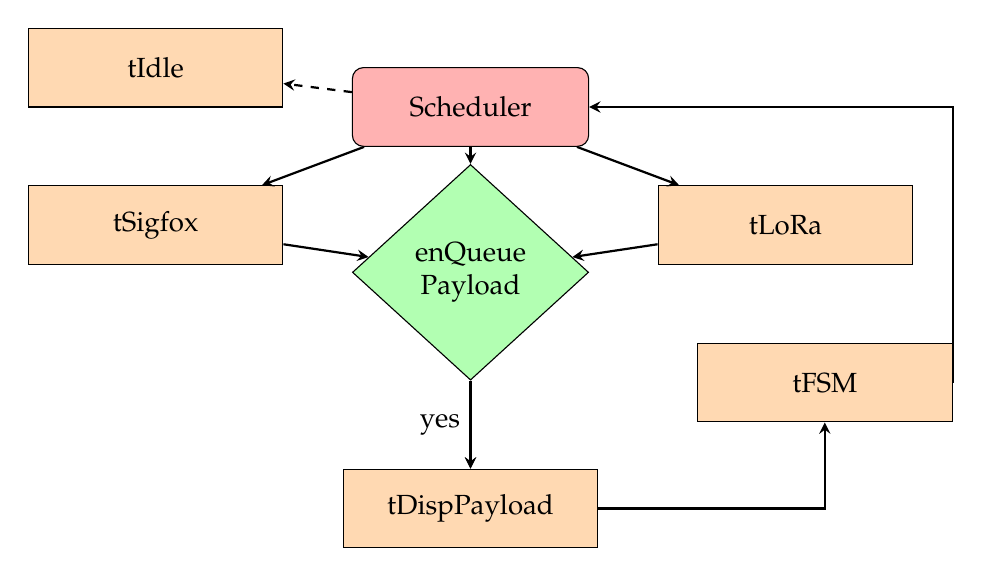
\begin{tikzpicture}[node distance=2cm]
\node (start) [startstop] {Scheduler};
%\node (in1) [io, below of=start] {lala};
\node (tSigfox) [process, left of=start, xshift=-2cm, yshift =-1.5cm] {tSigfox};
\node (tLoRa) [process, right of=start, xshift=2cm, yshift=-1.5cm] {tLoRa};
\node (dec1) [decision, below of=start, yshift=-0.1cm] {enQueue Payload};
\node (tIdle) [process, above of=tSigfox, yshift=0cm] {tIdle};
\node (tFSM) [process, below of=tLoRa, yshift= 0cm, xshift=0.5cm] {tFSM};
\node (tDisp) [process, below of=dec1, yshift=-1cm] {tDispPayload};


 \draw [arrow] (start) -- (tSigfox);
 \draw [arrow] (start) -- (dec1);
 \draw [arrow] (start) -- (tLoRa);
 \draw [arrow] (tSigfox) -- (dec1);
 \draw [arrow] (tLoRa) -- (dec1);
 \draw [arrow,dashed] (start) -- (tIdle);
 %\draw [arrow,dashed] (start) -| (tFSM.east);
 \draw [arrow] (tFSM.east) |- (start);
 \draw [arrow] (dec1) -- (tDisp);
\draw [arrow] (tDisp) -| (tFSM);
 

\draw [arrow] (dec1) -- node[anchor=east] {yes} (tDisp);
% \draw [arrow] (dec1) -- node[anchor=south] {no} (pro2b);

\end{tikzpicture}
\caption{Diagrama de tareas}
\label{fig:Diagrama de flujo}
\end{figure}

\subsubsection{Comunicación con el modulo Sigfox}
La tarea tSigfox se encarga de iniciar el servicio de comunicación con el módulo Sigfox, Le envía los comandos necesarios de configuración para dejarlo listo para trabajar, cuando se configura se deshabilita la tarea.

\subsubsection{Comunicación con el modulo LoRaWAN}
Esta tarea se encarga de iniciar el servicio de comunicación con el módulo LoRa, Le envía los comandos necesarios de configuración para dejarlo listo para trabajar, se basa en una corutina, cuando se configura se deshabilita la tarea.

\subsubsection{Lectura de entradas analógicas y digitales}
Esta tarea se encarga de muestrear periódicamente las señales analógicas y digitales.

\subsubsection{Despachador de mensajes}
Es una tarea que esta asociada a una cola de eventos. Esta tarea se dispara cada vez que hay un mensaje para transmitir en la cola.
\\
\newline
\newline
\newline
\newline
\hfill \break
\subsubsection{Tarea para una FSM (\textit{Finite State Machine})}
Esta tarea se encarga de realizar la secuencia de inicializar variables del sistema, enviar el mensaje por Sigfox o por LoRaWAN y colocar el módulo en modo de bajo consumo, la secuencia se repite periódicamente. En la figura \ref{fig:DiagramadeFSM} se puede observar la secuencia.

\begin{figure}[H]
\centering
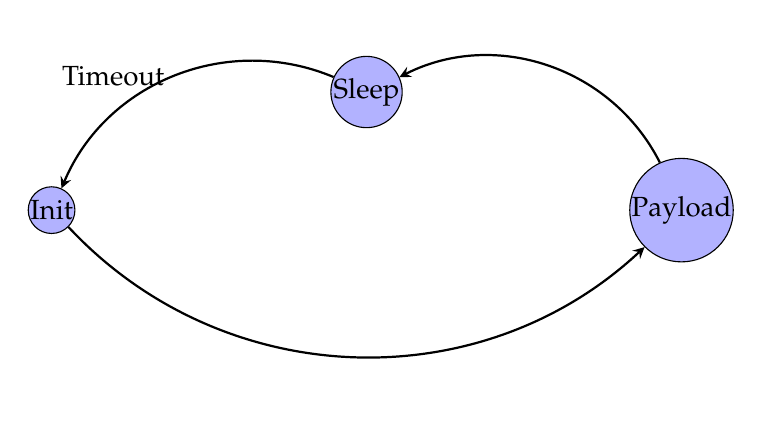
\begin{tikzpicture}[node distance=2cm]
\node (start) [fsm] { Sleep };
%\node (in1) [io, below of=start] {lala};
\node (init) [fsm, left of=start, xshift=-2cm, yshift =-1.5cm] {  Init  };
\node (payload) [fsm, right of=start, xshift=2cm, yshift=-1.5cm] {Payload};

 \draw [arrow] (start) to [bend right=45] node[anchor=east] {Timeout} (init);
 \draw [arrow] (init) to [bend right=45]  (payload);
 \draw [arrow] (payload) to [bend right=45]  (start);



% \draw [arrow] (dec1) -- node[anchor=south] {no} (pro2b);

\end{tikzpicture}
\caption{Diagrama de la FSM}
\label{fig:DiagramadeFSM}
\end{figure}


% Chapter Template

\chapter{Ensayos y Resultados} % Main chapter title

\label{Chapter4} % Change X to a consecutive number; for referencing this chapter elsewhere, use \ref{ChapterX}

%----------------------------------------------------------------------------------------
%	SECTION 1
%----------------------------------------------------------------------------------------

En esta sección se presentan los ensayos realizados, los resultados obtenidos y el análisis correspondiente.

\section{Dispositivos desarrollados}
En la figura \ref{fig:MainBoaard} se puede observar el resultado del diseño de la tarjeta. Esta se encuentra armada con los módulos insertables Sigfox y LoRa y fue sometida a diferentes ensayos indicados en la sección \ref{sec:pruebasHW} 

\begin{figure}[H]
	\centering
	\includegraphics[scale=.45]{./Figures/MainBoardCompleta.jpeg}
	\caption{Tarjeta principal armada con los módulos Sifox y LoRa.}
	\label{fig:MainBoaard}
\end{figure}


\section{Pruebas de hardware sobre el prototipo} \label{sec:pruebasHW}
A la tarjeta se le hicieron pruebas individuales de hardware:
\begin{itemize}
    \item Cortos y continuidades.
    \item Voltaje en la linea de alimentación.
    \item Test visual comparado con el plano de ensamble, (ver figura
    \ref{fig:Planoensamble}.)
\end{itemize}

\begin{figure}[H]
	\centering
	\includegraphics[scale=.45]{./Figures/Planoensamble.PNG}
	\caption{Plano de ensamble tarjeta principal.}
	\label{fig:Planoensamble}
\end{figure}

\section{Resultados de sintonización y verificación de la antena Sigfox}
En la ecuación \ref{eq:Impedancia2} y \ref{eq:Impedancia3} se pueden observar los valores de la impedancia y RL medidos con el VNA para una frecuencia de 915.516625 MHz.

En la figura \ref{fig:tunnigsigfoxchart} se puede observar el resultado de la verificación de la antena con el VNA, donde el marcador se encuentra muy cerca al origen de la carta de Smith y al eje real. Lo ideal en la sintonización es que el valor de la resistencia se acerque a \SI{50}{\ohm} y el valor de la reactancia (parte imaginaria \textit{j} de la ecuación \ref{eq:Impedancia2}) sea lo mas cercano a \SI{0}{\ohm} para garantizar la mejor eficiencia y la menor reflexión posible.

En la figura \ref{fig:tunnigsigfox5} se puede observar los resultados de la curva de perdidas de retorno. Esta deja evidenciar que tiene un ancho de banda de aproximadamente 125 KHz, el cual se mide a partir de -10dB\citep{AntenaSigFox2016}.


\begin{equation}
	\label{eq:Impedancia2}
	Z = 37.5\SI{}{\ohm} - j*4.7\SI{}{\ohm}
\end{equation}
\begin{equation}
	\label{eq:Impedancia3}
    RL = -16.35 dB
\end{equation}

\begin{figure}[H]
	\centering
	\includegraphics[scale=.7]{./Figures/tunnigsigfoxchart.png}
	\caption{Carta de Smith 915 MHz.}
	\label{fig:tunnigsigfoxchart}
\end{figure}

\begin{figure}[H]
	\centering
	\includegraphics[scale=.35]{./Figures/tunnigsigfox5.png}
	\caption{Perdidas de retorno a 915 MHz.}
	\label{fig:tunnigsigfox5}
\end{figure}


%  Este valor de impedancia se encuentra muy cercano al eje real (37.5\SI{}{\ohm}). Entre mas cercano al eje real  y el valor de la reactancia X sea lo mas cercano a 0\SI{}{\ohm} habrán menos perdidos por reflexión. 


\section{Resultados de pruebas funcionales sobre  los módulos}

Los módulos Sigfox y LoRa se probaron individualmente, enviándole comandos AT y comandos MAC respectivamente. Con esto se verificó la correcta funcionalidad del dispositivo.
%y la verificación de consumos de corriente en modo \textit{Sleep}. 

% \begin{figure}[H]
% 	\centering
% %	\includegraphics[scale=.45]{./Figures/CartaSmith.png}
% 	\caption{Consumo de corriente modulo Wisol - Sigfox.}
% 	\label{fig:ConsumoWisol}
% \end{figure}

% \begin{figure}[H]
% 	\centering
% %	\includegraphics[scale=.45]{./Figures/CartaSmith.png}
% 	\caption{Consumo de corriente modulo RN2903 - LoRaWAN.}
% 	\label{fig:ConsumoLoraWAN}
% \end{figure}
\subsubsection{Resultados de las pruebas de transmisión de Sigfox}
Para la verificación de las transmisiones se uso el \textit{Back-end} Sigfox para la visualización de los paquetes de datos enviados.

En la figura \ref{fig:COMANDOSATSIGFOX} se pueden observar los comandos enviados al modulo Sigfox. En la figura \ref{fig:tRANSMISIONsIGFOX} se puede observar el mensaje de prueba visto en la plataforma de Sigfox. También se visualiza la cantidad (15) de estaciones bases que vieron el dispositivo y la cantidad de reenvíos (\textit{frames}), en 9 de 15 antenas se recibieron 3 de 3 paquetes enviados, por defecto Sigfox  envía tres \textit{frames} en cada transmisión y cada antena los recibe dependiendo de lo alejado que se encuentre el dispositivo de la estación base.

\begin{figure}[H]
	\centering
	\includegraphics[scale=.5]{./Figures/COMANDOSATSIGFOX.PNG}
	\caption{Comandos enviados al módulo Wisol-Sigfox.}
	\label{fig:COMANDOSATSIGFOX}
\end{figure}
\begin{figure}[H]
	\centering
	\includegraphics[scale=.35]{./Figures/tRANSMISIONsIGFOX.PNG}
	\caption{Prueba de transmisiones de mensajes de subida Sigfox.}
	\label{fig:tRANSMISIONsIGFOX}
\end{figure}

El dispositivo se alejo 10 Km del lugar de donde inicialmente se realizaron las transmisiones. En la figura \ref{fig:AntenasSigfoxAlejada} se puede observar que la cantidad (8 a 10) de estaciones base que vieron el dispositivo.
\begin{figure}[H]
	\centering
	\includegraphics[scale=.45]{./Figures/AntenasSigfoxAlejada.PNG}
	\caption{Transmisiones de mensajes Sigfox a 10Km de distancia.}
	\label{fig:AntenasSigfoxAlejada}
\end{figure}

\subsubsection{Resultados de las pruebas de transmisión de LoRaWAN}

En la figura \ref{fig:ComandMacLora} se pueden observar los comandos enviados al modulo LoRaWAN. Para la verificación de las transmisiones de loRaWAN se usó el servidor \textit{the things network} para la visualización de los paquetes de datos enviados (ver figura \ref{fig:Datalorawantest}).


\begin{figure}[H]
	\centering
	\includegraphics[scale=.45]{./Figures/ComandMacLora.PNG}
	\caption{Comandos enviados al módulo LoRaWAN.}
	\label{fig:ComandMacLora}
\end{figure}
\begin{figure}[H]
	\centering
	\includegraphics[scale=.35]{./Figures/Datalorawantest.PNG}
	\caption{Prueba de transmision de mensajes con LoRaWAN.}
	\label{fig:Datalorawantest}
\end{figure}

En la figura \ref{fig:LoraTX_corto} se puede observar que de 156 mensajes transmitidos con el dispositivo a una distancia menor a 1m del gateway. Solo 6 mensajes fueron recibidos por el servidor.
\begin{figure}[H]
	\centering
	\includegraphics[scale=.5]{./Figures/LoraTX_corto.PNG}
	\caption{Cuantificación de mensajes enviados con LoRaWAN.}
	\label{fig:LoraTX_corto}
\end{figure}
%\footnotetext{\url{https://www.thethingsnetwork.org/}}

\section{Pruebas de consumo de energía}
Los módulos LoRaWAN y Sigfox trabajan bajo redes LPWAN, por lo que el consumo debe ser lo más bajo posible. Esto debido a que en las aplicaciones se busca que los dispositivos finales tengan una durabilidad de muchos años. En la tabla \ref{tab:ConsumosTabla} se pueden observar los datos de los consumos usados.

\begin{table}[h]
	\centering
	\caption[Consumos]{Medición de consumos energéticos Sigfox y LoRaWAN }
	\begin{tabular}{l c c}    
		\toprule
		\textbf{ \textit{Modo} } & \textbf{Sigfox} & \textbf{LoRaWAN} \\
		\midrule
		Normal	    &$\mathrm{0.53 mA}$ 	&$\mathrm{6.71 mA}$  \\	
		\textit{Sleep}	            & $\mathrm{0.3 \mu{A}}$     & $\mathrm{6.4 \mu{A}}$\\
		\bottomrule
		\hline
	\end{tabular}
	\label{tab:ConsumosTabla}
\end{table}


El consumo energético del modulo Sigfox WWSFM11R2D se puede observar en la figura \ref{fig:Consumo_SigNormal} y \ref{fig:ConsumoSigSleep}. 
\begin{figure}[H]
	\centering
	\includegraphics[scale=.15]{./Figures/Consumo_SigNormal.jpeg}
	\caption{Consumo de WWSFM11R2D en funcionamiento normal.}
	\label{fig:Consumo_SigNormal}
\end{figure}

\begin{figure}[H]
	\centering
	\includegraphics[scale=.15]{./Figures/ConsumoSigSleep.jpeg}
	\caption{Consumo de WWSFM11R2D en modo \textit{sleep}}
	\label{fig:ConsumoSigSleep}
\end{figure}

El consumo energético del modulo LoRaWAN se puede observar en la figura \ref{fig:ConsumoLoraNormal} y \ref{fig:ConsumoLoraSleep}. 

\begin{figure}[H]
	\centering
	\includegraphics[scale=.15]{./Figures/ConsumoLoraNormal.jpeg}
	\caption{Consumo de RN2903 en funcionamiento normal.}
	\label{fig:ConsumoLoraNormal}
\end{figure}

\begin{figure}[H]
	\centering
	\includegraphics[scale=.15]{./Figures/ConsumoLoraSleep.jpeg}
	\caption{Consumo de RN2903 en modo \textit{sleep}}
	\label{fig:ConsumoLoraSleep}
\end{figure}

La medición de corriente en los módulos deja evidenciar que mientras se encuentra en modo de funcionamiento el consumo es alto, sin embargo cuando se les envía el comando para entrar en modo de bajo consumo la corriente baja considerablemente al orden de $\mu{A}$.


\section{Pruebas de integración}
Para las pruebas de integración se contó con :
\begin{itemize}
    \item Acceso remoto al servidor de Sigfox y LoRaWAN. 
    \item Acceso remoto a  la plataforma xxxx para no visualizar las señales en crudo.
    \item Acceso físico a los dispositivos embebidos
    \item Terminal serial WCOM desarrollada por Tecrea SAS.
    \item Multimetro UNI-T ut61D con resolución de hasta 100 nA.
    \item Acceso a consola serial de la tarjeta principal.
\end{itemize}

En la figura \ref{fig:IntegracionSL2} se puede observar la consola de depuracíon del dispositivo. Durante el proceso de pruebas permitió la visualización del estado interno de la aplicación embebida al mostrar los mensajes impresos por el firmware desarrollado. Se puede visualizar que el mensaje enviado es:

00 00 00 00 00 00 06 00 02 AB 09 c7 

Este se puede decodificar de acuerdo a la siguiente imagen \ref{fig:FRAME}, como cada canal analógico es de 12 bits, al valor de los canales ADC0, ADC1, ADC2 se les debe aplicar la formula \ref{eq:ADC} para obtener el resultado de 2.786 V, 4.5 V y 0 mA.

\begin{equation}
	\label{eq:ADC}
	VADCx = (ADCx -2340 ) / 58.5
\end{equation}

\begin{figure}[H]
	\centering
	\includegraphics[scale=.6]{./Figures/FRAME.PNG}
	\caption{Codificación del paquete de datos.}
	\label{fig:FRAME}
\end{figure}

\begin{figure}[H]
	\centering
	\includegraphics[scale=.6]{./Figures/IntegracionSL2.PNG}
	\caption{Consola de depuración del sistema embebido.}
	\label{fig:IntegracionSL2}
\end{figure}


En la figura \ref{fig:Ubidotsintegration} se puede observar la visualización del \textit{dashboard} con la medición de las variables en la plataforma Ubidots.

\begin{figure}[H]
	\centering
	\includegraphics[scale=.3]{./Figures/Ubidotsintegration.PNG}
	\caption{Plataforma de integración.}
	\label{fig:Ubidotsintegration}
\end{figure}

%\section{Pruebas unitarias de manejadores de dispositivos (\textit{driver})}








 
% Chapter Template

\chapter{Conclusiones} % Main chapter title

\label{Chapter5} % Change X to a consecutive number; for referencing this chapter elsewhere, use \ref{ChapterX}


%----------------------------------------------------------------------------------------

%----------------------------------------------------------------------------------------
%	SECTION 1
%----------------------------------------------------------------------------------------
En este capítulo se destacan los principales aportes al trabajo realizado, se evalúa el cumplimiento de los requerimientos y se destacan los conocimientos aplicados.
\section{Conclusiones generales del trabajo realizado}


Los principales resultados del trabajo realizado son los siguientes:

\begin{itemize}
    \item Se logró construir un prototipo de hardware principal y un prototipo por cada uno de los dos módulos de comunicación de acuerdo al objetivo establecido.
    \item A partir de los resultados presentados en el capitulo \ref{Chapter4} se puede afirmar que no es necesario realizarle una sintonización a la antena externa que lleva el dispositivo, debido a que cumple con los parámetros teóricos y empíricos mencionados en la sección \ref{subseccionAntena}
\end{itemize}


\begin{itemize}
    \item Se concluye además de acuerdo a las mediciones realizadas que el modulo Sigfox consume menos energía en modo normal y en bajo consumo que el modulo LoRaWAN. esto permite que pueda ser útil en muchas aplicaciones donde lo primordial es la durabilidad de la batería del dispositivo.
    \item El consumo de los dispositivos se puede ver afectado por un ensamble defectuoso, como exceso de soldadura o soldaduras en frió. Se debe garantizar que los pines sobrantes en el microcontrolador se coloque como entradas analógicas (alta impedancia) y también se deben garantizar los niveles lógicos de las entradas digitales. Cabe aclarar que estas son conclusiones que se dan de acuerdo a la experiencia con el manejo de dispositivos de bajo consumo y el desarrollo del presente trabajo. Sin embargo se debe siempre acudir a la hoja de datos y recomendaciones del fabricante.
\end{itemize}

\begin{itemize}
    \item Para decidir cual de las dos tecnologías (Sigfox o LoRa) a usarse debe analizar el caso de uso y la región, por que por ejemplo en Colombia  no hay un gran proveedor de la red LoRa como si lo tiene Sigfox. Sin embargo hay quienes prefieren montar el servidor y la red con LoRa ellos mismos y hay otras personas que prefieren tener todo a la mano como se lo brinda Sigfox. En otros países donde la red loRa tiene mas despliegue, quizás Sigfox no sea la mejor opción, debido a que en LoRa se puede tener una mejor transferencia de datos y mejor confirmación con mensajes de subida. En los mensajes de bajada no tiene la restricción de 120 mensajes mensuales como si lo tiene Sigfox.
    \item De acuerdo a los resultados de las transmisiones con LoRaWAN, se tiene que de los mensajes transmitidos solo el 3.85 \% de ellos llegaron al servidor, esto debido a que el gateway que se tenía disponible era de un solo canal y no era el optimo para este uso.
\end{itemize}


\subsection{Cumplimiento de los requerimientos}

Todos los requerimientos se implementaron de forma exitosa. Sin embargo de acuerdo a las sugerencias del director se decidió enfocar el proyecto una de las dos tecnologías, en este caso Sigfox debido a que se presentaron inconvenientes en la adquisición del gateway LoRa, sin embargo se lograron realizar algunas transmisiones con un gateway LoRa de un solo canal obtenido a ultimo momento.

Cabe mencionar que el inconveniente mas relevante fue el no poder tener un gateway apropiado en el momento necesario.

\subsection{Conocimientos utilizados}
Para el desarrollo de este trabajo se utilizaron los siguientes conocimientos.

\begin{itemize}
\item Programación de microprocesadores: se aprovecha la experiencia adquirida en lenguaje C en microcontroladores con arquitecturas de 32 bits y se aplica a otro microcontroladores como lo es STM32.
\item Gestión de proyectos: El aporte de esta asignatura contribuyo considerablemente en el desarrollo de un plan de trabajo claro y organizado, permitiendo que el desarrollo del proyecto se ejecutara de la mejor manera.
\item Protocolos de comunicación en sistemas embebidos: Se aplicaron los conocimientos para la programación de los periféricos I2C y UART. También se aplicaron los conocimientos de desarrollo de manejadores de dispositivos en los drivers del modulo Sigfox y LoRaWAN.
\item Sistemas Operativos de Tiempo Real (I y II) : Con estas asignaturas se desarrollo una mejor perspectiva de los sistemas concurrentes en sistemas embebidos y fue muy útil en el desarrollo del firmware del proyecto, ya que se uso un sistema operativo cooperativo .
\end{itemize}

También se adquirieron conocimientos en:
\begin{itemize}
    \item Configuración de módems.
    \item Trasmisión de datos a plataformas integradoras pagas y \textit{open source}.
    \item Control de versiones.
    \item Test de pruebas unitarias.
\end{itemize}

Y se aplicaron conocimientos previamente adquiridos como:
\begin{itemize}
    \item \textit{Testing} y control de calidad en los circuitos.
    \item Diseño electrónico y de PCB.
    \item Diseño de antenas.
    \item Sintonización de antenas.
    \item Desarrollo de firmware y manejadores de dispositivos orientado a objetos.
\end{itemize}


%----------------------------------------------------------------------------------------
%	SECTION 2
%----------------------------------------------------------------------------------------
\section{Trabajo futuro}

Para el futuro del proyecto se propone trabajar con las tecnologías NB-IoT, CAT-M1 ó GSM. Hay algunos módulos como el BG96 de la marca Quectel que incorpora estas dos tecnologías de comunicación, 2G y GPS. Sin embargo,por costos también se puede trabajar estas tecnologías en módulos individuales, ya que el dispositivo de adquisición de datos permite acoplarlo fácilmente, simplemente diseñando una tarjeta con el conector adecuado y que se pueda comunicar por UART o I2C. 


% En la figura \ref{fig:gsm1} y \ref{fig:gsm} se puede observar el módulo UC20 fabricado por la empresa Quectel, este trabaja bajo la red 2G, 3G y tiene GPS interno.


% \begin{figure}[H]
% 	\centering
% 	\includegraphics[scale=.45]{./Figures/gsm1.jpeg}
% 	\caption{Vista frontal del módulo 2G y 3G insertable.}
% 	\label{fig:gsm1}
% \end{figure}

% \begin{figure}[H]
% 	\centering
% 	\includegraphics[scale=.45]{./Figures/gsm.jpeg}
% 	\caption{Vista posterior del módulo 2G y 3G insertable.}
% 	\label{fig:gsm}
% \end{figure}
 

%----------------------------------------------------------------------------------------
%	CONTENIDO DE LA MEMORIA  - APÉNDICES
%----------------------------------------------------------------------------------------

\appendix % indicativo para indicarle a LaTeX los siguientes "capítulos" son apéndices

% Incluir los apéndices de la memoria como archivos separadas desde la carpeta Appendices
% Descomentar las líneas a medida que se escriben los apéndices

%\input{Appendices/AppendixA}
%\input{Appendices/AppendixB}
%\input{Appendices/AppendixC}

%----------------------------------------------------------------------------------------
%	BIBLIOGRAPHY
%----------------------------------------------------------------------------------------

\Urlmuskip=0mu plus 1mu\relax
\raggedright
\printbibliography[heading=bibintoc]

%----------------------------------------------------------------------------------------

\end{document}  
